\documentclass[12pt,aip,cha,reprint,nofootinbib]{revtex4-1}
\usepackage{amsfonts,amssymb,amsmath,times}%
\usepackage{graphicx}
\usepackage{bm}
\usepackage{enumerate}
\usepackage{color}

% \linespread{1}

\begin{document}

\title{Characterizing dynamical transitions by statistical complexity measures based on ordinal pattern transition networks} 

\author{Min Huang}
	\affiliation{School of Physics and Electronic Science, East China Normal University, Shanghai 200062, China}

\author{Zhongkui Sun}
	\affiliation{Department of Applied Mathematics, Northwestern Polytechnical University, Xi'an 710072, China}

\author{Jie Zhang}
	\affiliation{Institute of Science and Technology for Brain-Inspired Intellegence, Fudan University, Shanghai 200433,  China}

\author{Reik V. Donner}
        \affiliation{Department of Water, Environment, Construction and Safety, Magdeburg--Stendal University of Applied Sciences, Breitscheidstra{\ss}e 2, 39114 Magdeburg, Germany}
        \affiliation{Potsdam Institute for Climate Impact Research (PIK) -- Member of the Leibniz Association, Telegrafenberg A31, 14473 Potsdam, Germany}

\author{Shuguang Guan}
	\email[corresponding author: ]{sgguan@phy.ecnu.edu.cn}
	\affiliation{School of Physics and Electronic Science, East China Normal University, Shanghai 200062, China}
	
\author{Yong Zou}
	\email[corresponding author: ]{yzou@phy.ecnu.edu.cn}
	\affiliation{School of Physics and Electronic Science, East China Normal University, Shanghai 200062, China}

\date{\today}

\begin{abstract}
Complex network approaches have been recently emerging as novel and complementary concepts of nonlinear time series analysis which are able to unveil many features that are hidden to more traditional analysis methods. In this work, we focus on one particular approach: the application of ordinal pattern transition networks for characterizing time series data. More specifically, we generalize some traditional estimators of statistical complexity measures (SCMs), which explicitly disclose heterogeneous frequencies of ordinal pattern transitions in the time series networks. To demonstrate the usefulness of the estimators, we employ SCMs to characterize different dynamical transitions in the logistic map as a paradigmatic model system, as well as real-world time series of fluid experiments and ECG data. The obtained results for both, artificial and experimental data demonstrate that the consideration of transition frequencies between different ordinal patterns leads to dynamically meaningful estimates of SCMs, which provide prospective tools for the analysis of time series with finite length. 
\end{abstract}

\pacs{05.45.Ac, 05.45.Tp, 89.75.Fb}
\maketitle

\begin{quotation}
In the recent decade, traditional tools of nonlinear time series analysis have been undergoing fast developments benefiting from concepts from complex network theory. Along this line of research topics, ordinal pattern transition networks have been expanding the established concept of permutation entropy and provide complementary insights into the dynamical organization underlying time series data. Traditionally, permutations based on order patterns are simple and easy to implement concepts providing estimators of statistical complexity measures (SCMs), which however rely on static pattern frequencies only. Yet, much additional information can be exploited by including order pattern transitions into the definitions of SCMs -- an idea that however has not been widely developed and applied so far. In this work, we generalize existing estimators of SCMs by means of ordinal pattern transition networks which take into account the pattern transition properties explicitly. The usefulness of our generalizations of existing SCMs is demonstrated by using time series of both, model and experimental data. 
\end{quotation}

\section{Introduction}
In the recent decade, complex network based approaches have emerged as prominent tools for nonlinear time series analysis \cite{Kantz97,Sprott2003}, which have found many interesting applications to experimental data from various origins \cite{ZouPR2018}. In this line of research, there exist several major methods that are of particular importance, including recurrence networks \cite{MarwanPLA2009,Donner2010a}, visibility graphs \cite{Lacasa2008,Nunez2012}, transition networks \cite{Nicolis2005,MichaelChaos2015} and cycle networks \cite{ZhangPRL2006}. Depending on the particular questions at hand, each of these complex network approaches exhibit various variants that can be employed for different application purposes. For instance, we may either construct a single network representing a univariate time series, or interacting, multiplex or multi-layer networks for coupled time series. For a recent systematic review, see Ref.~\cite{ZouPR2018}. In this work, we focus on constructing ordinal pattern transition networks (OPTNs) for time series data, which present the advantages of easy implementation and a wide range of existing application to data from different origins, including correlated stochastic processes, neurophysiological (EEG) and human cardiac activity (ECG) series \cite{MichaelChaos2015,KulpChaos2016,zhangSciRep2017,McCullough2017b,BorgesAMC2019,Subramaniyam2020}. 

The basic idea behind the OPTN method originates from identifying ordinal patterns in time series \cite{BandtPRL2002}, which is a well developed concept in nonlinear time series analysis leading to, for instance, the widely employed measure of permutation entropy \cite{BandtPRL2002}. In addition, ordinal symbolic representations of time series have found a number of interesting applications in science and engineering, for instance, in biomedical recordings \cite{AmigoPTRSA2014}, finance \cite{ZaninChaos2008}, and even climate \cite{BarreiroChaos2011}. Some recent progress has been comprehensively reviewed in Ref.~\cite{AmigoPTRSA2014}. 

More specifically, given a one-dimensional time series $\{ x_i\}_{i=1, \cdots, L}$ comprising $L$ observations from a dynamical system, we first reconstruct the corresponding phase space by time delay embedding $\vec{x}_i = [x_i, x_{i+\tau}, \ldots, x_{i+(D-1)\tau}]$ with an embedding dimension $D$ \cite{Takens1981,Kantz97}. Next, we represent each embedding vector $\vec{x}(i)$ by the corresponding rank order of its components, which is encoded into a symbol $\pi_{i}$. Hence, when sliding windows from $i=1$ to $N = L - (D - 1)\tau$ in the embedding space, a symbolic representation of the trajectory $\{\pi_i\}$ is produced. It is possible to derive information about the dynamics of the underlying system by assessing the probabilities of occurrence of different ordinal patterns. For example, for time series resulting from deterministic dynamical systems, certain patterns may not occur at all. More generally, we obtain an empirical probability distribution $P$ whose elements $p_{\pi_{i}}$ are the frequencies associated to the different patterns $\pi_{i}$, $i = 1, \cdots, D!$. Clearly, $P$ provides a significant and feasible way to estimate a characteristic probability distribution function for a given time series, which plays a crucial role in extracting statistical complexity information on the underlying dynamical systems \cite{BandtPRL2002,AmigoPTRSA2014}. 

The conceptually relatively simple computation of $P$ based on ordinal patterns for the underlying system prompts to another successful application of this framework in terms of statistical complexity measures (SCMs) \cite{kowalskiEntropy2011}. One common way of defining SCMs is taking the product of a normalized Shannon entropy and an associated measure of disequilibrium \cite{LopezPLA1995,kowalskiEntropy2011}, which captures specific organizational properties of structure and patterns in a process. Following the vast amount of previous work on this topic  \cite{rossoPRL2007,LopezPLA1995,kowalskiEntropy2011,Lange2013}, in this work we consider a variant of SCMs based on the concept of Jensen-Shannon divergence, which is defined as $\mathcal{C}_{JS}[P] = \mathcal{H}[P] \cdot  Q_{JS}[P, P_e]$, where $\mathcal{H}[P]$ is the normalized Shannon entropy and $Q_{JS}[P, P_e]$ is the so-called disequilibrium function measuring the distance of the given distribution $P$ to the uniform distribution $P_e$. Accordingly, we define $Q_{JS}[P, P_e] = Q_{0} \cdot JS[P, P_e]$ where $JS[P, P_e]$ is the Jensen-Shannon divergence between $P$ and $P_e$ and $Q_{0}$ is a normalization factor. Furthermore, the complexity--entropy plane $\mathcal{H} \times \mathcal{C}_{JS}$ has been intensively used to distinguish chaotic systems from stochastic ones \cite{rossoPRL2007}. The analysis of complexity--entropy planes has already taken advantage from the ordinal pattern based symbolic encoding of time series and has found various applications \cite{rossoPRL2007,kowalskiEntropy2011}. However, in the complexity--entropy analysis, there are some chaotic maps that could be easily confused with random noise because no clearly separable domains of values are available to differentiate those different types of dynamics as reported in \cite{BorgesAMC2019}. So far, it remains a challenging task to disclose a possible non-monotonic relationship between complexity and entropy \cite{MartinPLA2003}. 

It may be noted that in the above discussion on ordinal pattern based time series analysis methods, the transition behavior between patterns has largely remained unconsidered. Recently, OPTN representations have been proposed to precisely capture this transition behavior of the ordinal patterns \cite{MichaelChaos2015,KulpChaos2016,zhangSciRep2017,McCullough2017b,BorgesAMC2019}, which opens a broader perspective beyond the standard ordinal symbolic analysis of time series. In this framework, each ordinal pattern is considered as a vertex in a graph, and a directed and weighted edge connecting two patterns in the graph is established according to the corresponding transition frequency (i.e., the probability with which a given permutation is followed by a certain other one). One of the advantages of the resulting OPTNs is that we can obtain a pronounced distinction between different types of systems based on short time series only \cite{MichaelChaos2015,BorgesAMC2019}. 

In this work, we draw upon the recent success of both, complexity--entropy plain analysis and OPTNs, to generalize the traditional SCMs by incorporating pattern transition probabilities. The advantages of this approach are as follows: (i) All SCMs successfully show clear distinction between different types of dynamics, which is demonstrated for time series from numerical models and experimental data. (ii) The generalized SCMs help to capture a consistent relationship between SCMs and chaoticity. (iii) All SCMs are sensitive to dynamical transitions along a bifurcation scenario, including period doubling, band merging, inner and outer crises. 

The remainder of this paper is organized as follows: In Section~\ref{sec:methods}, we introduce the methodology employed in our work. We start by discussing two slightly different ways to obtain the transition matrix between ordinal patterns, which provides the basis for defining the corresponding OPTNs (Section~\ref{sec:OPW}). Based on this matrix, we propose in Section~\ref{sec:SCM} to compute SCMs from three different perspectives, including static pattern frequency properties, dynamic pattern transition properties, and a combination of both. In Section~\ref{sec:results1}, we then proceed with describing some selected results for the logistic map as as paradigmatic model system exhibiting various types of periodic and chaotic solutions. We first discuss in some detail one example of a periodic orbit to emphasize the important effects of embedding parameters in Section~\ref{sec:embeddings}. The practical usefulness of SCMs will be further illustrated by studying four exemplary time series from different typical dynamical regimes (Section~\ref{sec:four}). In Section~\ref{sec:plane}, the complexity--entropy planes associated with each SCM will be discussed while the control parameter of the logistic map is systematically increased. In order to characterize the dynamical transitions in this model, we further study the behavior of the SCM values in dependence on the control parameter in Section~\ref{sec:transi} and show that similar results can also be obtained for time-continuous dynamical systems like the R\"ossler oscillator in Section~\ref{sec:cont}. Finally, we show that SCMs successfully distinguish different dynamical regimes in experimental time series from flow data and human ECG measurements in Section~\ref{sec:time}. Some concluding remarks and discussions will be provided in Section~\ref{sec:con}.  

\section{Methods} \label{sec:methods}

\subsection{Ordinal pattern transition matrix} \label{sec:OPW}

Most recent studies employing the concept of permutation entropy $\mathcal{S}_O$ have defined this measure by focusing exclusively on the frequencies of ordinal patterns, which however disregards the transition behavior between subsequent patterns. To emphasize the transition frequencies between any pair of patterns, measures of transitional complexity have been further proposed in Refs.~\cite{zhangSciRep2017,McCullough2017b} to quantify the properties of the associated OPTNs. To this end, we associate each directed link in an OPTN with its transition frequency $w_{ij} = p({\pi_i \to \pi_j})$. Calculating the transition frequencies for each pair of patterns, we obtain a weighted directed network characterized by a weighted adjacency matrix $\mathbf{W} = \{ w_{ij} \}, i, j \in [1, D!]$. 

Based on this transition matrix $\mathbf{W}$ of an OPTN, we note that there two slightly different ways to introduce normalization factors. The first option is to use a global normalization to ensure $\sum_{i,j}^{D!} w_{ij} = 1$ \cite{zhangSciRep2017}, which results in a globally normalized transition entropy as discussed below. The second option has been proposed by McCullough {\textit{et al}}~\cite{McCullough2017b} who first considered the local out-link transition frequency from pattern $\pi_i$ to $\pi_j$
\begin{equation} \label{eq:localTp}
p_{\pi_i \to \pi_j} = \left \{ \begin{aligned}
				& 0,  \;\;\;\;\;\;\;\;\;\;\;\;\;\;\;\;\;\;\;\;\; \text{if} \;\;\; \pi_i = \pi_j \\
				& \frac{w_{ij}}{\sum_{j, j \neq i} w_{ij}}, \;\;\;\;\;\; \text{if} \; \pi_i \neq \pi_j.\\
				\end{aligned}
				\right.
\end{equation}
\noindent
Note that the transition frequency of Eq.~\eqref{eq:localTp} is pattern (row-) wise normalized. This case will be referred to as the node-wise out-link normalized transition matrix $\mathbf{W}$ in the following. In this way, it easily captures the heterogeneous behavior of both (static) occurrence frequencies of different patterns and (dynamic) transition frequencies between patterns. 

In addition to the proper normalization, we need to consider self-loops that may affect the numerical estimation of $\mathbf{W}$ especially for time series from continuous systems with a given sampling rate. For example, it has been demonstrated in Ref.~\cite{zhangSciRep2017} that there are about $99\%$ self-loops in the time series of R\"ossler system when integrated with a step size $h = 0.01$, while the about $1\%$ non-self-loops are hidden in $\mathbf{W}$. From this example, one may easily see that self-loops are related to the serial correlation of the time series under study \cite{BorgesAMC2019}. On the other hand, neglecting self-loops in $\mathbf{W}$ emphasizes the transition behavior between different patterns, which has therefore been adopted in most existing studies of complex networks for computational simplicity and theoretical concerns \cite{CostaADPhy2007}. Accordingly, we also remove self-loops in the present study before computing the weighted matrix $\mathbf{W}$ while acknowledging that in other cases of stochastic processes and discrete systems, self-loops have been included in the analysis showing some interesting results \cite{BorgesAMC2019}. Arguably, whether to remove or to consider self-loops depends on the particular process under study. In any of the applications discussed in the rest of this paper, we have ensured that our results do not change qualitatively when considering the effects of self-loops.

\subsection{Statistical complexity measures} \label{sec:SCM}

In the following, we will briefly review the existing ordinal pattern frequency based SCM before proposing two novel ways to define SCMs, which explicitly consider transition frequencies of the resulting OPTN representations for time series. 
 
\subsubsection{SCM based on the permutation entropy of pattern frequencies} 

The permutation entropy of a time series is the Shannon entropy of the distribution of patterns $P = \{p_{\pi_1}, p_{\pi_2},\ldots,p_{\pi_i} \}$, which is defined as
\begin{equation}
\mathcal{S}_{O}[P]= - \sum_{i=1}^{D!} p_{\pi_i} \log p_{\pi_i}. 
\end{equation}
The normalized permutation entropy $\mathcal{H}_O$ hence follows as 
\begin{equation} \label{eq:Ho}
\mathcal{H}_{O}[P] = \mathcal{S}_{O}[P] / \mathcal{S}_{O, max}, 
\end{equation}
where $\mathcal{S}_{O, max} = \log D!$ corresponds to the case of a uniform distribution of the same number of patterns, i.e., $P_e = \{1/D!, \ldots, 1/D!\}$. 

In the next step, we use some appropriate statistical concept to measure the distance of the given empirical distribution $P$ to the uniform distribution $P_e$, which is the essential idea behind the class of SCMs considered in this work. Several different distance functions have been considered in the literature, including the Euclidean norm, Wooters' distance, Kullback-Leibler relative entropy and Jensen-Shannon divergence \cite{kowalskiEntropy2011}. In this work, the distance between the distributions $P$ and $P_e$ is characterized by the Jensen-Shannon divergence $Q_{JS}[P] = Q_0 \cdot JS[P, P_e]$ with 
\begin{equation}
JS[P, P_e] = \mathcal{S}_O[(P+P_e)/2] - \frac{1}{2}\mathcal{S}_O[P] - \frac{1}{2}\mathcal{S}_O[P_e], 
\end{equation}
where $Q_0$ is a normalization factor with equals the inverse of the maximal Jensen-Shannon divergence $JS[P, P_e]$, which ensures that $Q_{JS}[P] \in [0, 1]$. This maximal distance is obtained when the distribution $P$ has probability one for one pattern and zero for all other patterns. The general expression for $Q_0$ reads  
\begin{equation} \label{eq:Q0}
Q_0 = \frac{-2}{\left(\frac{N+1}{N}\right) \log (N+1) -2 \log (2N) + \log (N)},
\end{equation}
where $N = D!$ is the total number of possible patterns. For large $D$, we have $Q_0 \approx 1 /  \log 2$. 

The function $Q_{JS}[P]$ is different from zero if the system has a kind of preference of certain patterns among the accessible ones, reflecting determinism of the system. Finally, the SCM based on permutation entropy of node (pattern) frequencies is defined as 
\begin{equation}
\mathcal{C}_{O}[P] = Q_{JS}[P] \cdot \mathcal{H}_{O}[P].
\end{equation}
This quantity is static in the sense that it quantifies the amount of information stored by ordinal frequencies in the system and its disequilibrium of the observed parts of its accessible states in comparison to a uniform distribution \cite{LopezPLA1995}. 

\subsubsection{SCM based on the transition entropy of the globally normalized weight matrix} 

In this case, the sum of all entries of the transition matrix $\mathbf{W}$ is 1, and the Shannon entropy of transition frequencies between any pair of ordinal patterns is therefore 
\begin{equation}
\begin{split}
\mathcal{S}_{W}[W] &= - \sum_{i=1}^{D!} \sum_{j = 1; j \neq i}^{D!} w_{ij} \log w_{ij}, \\
& = - \sum_{i=1}^{D!} \sum_{j =1; j \neq i}^{D!} p_{\pi_i \to \pi_j} \log p_{\pi_i \to \pi_j}. 
\end{split}
\end{equation}
The normalized entropy is hence defined 
\begin{equation}
\mathcal{H}_{W}[W] = \mathcal{S}_{W}[W] / \mathcal{S}_{W, max}, 
\end{equation}
where $\mathcal{S}_{W, max} = \log D! (D! - 1)$ as any self transitions are excluded. Furthermore, there are $D! (D! - 1)$ possible pattern transitions in the uniformly distribution function $P_e$. Thus, in a full analogy with the node-based SCM, the Jensen-Shannon distance is computed as $Q_{JS}[W] = Q_0 \cdot JS[W, P_e]$ with
\begin{equation}
JS [W, P_e] = \mathcal{S}_{W}[(W + P_e)/2] - \frac{1}{2}\mathcal{S}_{W}[W] - \frac{1}{2}\mathcal{S}_{W}[P_e]. 
\end{equation}
We note that we have the same expression for the normalization factor $Q_0$ as above while replacing $N = D! (D! - 1)$ in Eq.~\eqref{eq:Q0}. This further yields the SCM 
\begin{equation}
\mathcal{C}_{W}[W] = Q_{JS}[W] \cdot \mathcal{H}_{W}[W].
\end{equation}
This quantity is dynamic in the sense that it considers the state transition information stored in the system. 

\subsubsection{SCM based on the transition entropy of the node-wise out-edge normalized weighting matrix}

We finally consider the case where the ordinal transition matrix is node-wised normalized, i.e., the row sum of $\mathbf{W}$ is 1. Accordingly, we again first introduce the node-wise out-edge transition entropy
\begin{equation}
\begin{split}
\mathcal{S}_{E}^{\pi_i}[W_{\pi_i}] &= - \sum_{j = 1; j \neq i}^{D!} w_{ij} \log w_{ij},  \\ 
&= - \sum_{j=1, j \neq i}^{D!} p_{\pi_i \to \pi_j} \log p_{\pi_i \to \pi_j} 
\end{split}
\end{equation}
and node-wise normalized transition entropy
\begin{equation}
\mathcal{H}_{E}^{\pi_i}[W_{\pi_i}] = \mathcal{S}_{E}^{\pi_i}[W_{\pi_i}] / \mathcal{S}_{E, max} 
\end{equation}
with $\mathcal{S}_{E, max} = \log (D! - 1)$. Note that this normalization factor is the same for all patterns, i.e., $\mathcal{S}_{E, max}^{\pi_i} = \mathcal{S}_{E, max}^{\pi_j}$. Therefore, the superscript index can be suppressed in the above definition. In addition, the node-wise Jensen-Shannon distance is defined as $Q_{JS}^{\pi_i}[W_{\pi_i}] = Q_0 \cdot JS^{\pi_i} [W_{\pi_i}, P_e]$ with the disequilibrium measure
\begin{eqnarray}
&&JS^{\pi_i} [W_{\pi_i}, P_e] = \nonumber \\
&&\quad \mathcal{S}_{E}^{\pi_i}[(W_{\pi_i} + P_e)/2] - \frac{1}{2}\mathcal{S}_{E}^{\pi_i}[W_{\pi_i}] - \frac{1}{2}\mathcal{S}_{E}^{\pi_i}[P_e]. 
\end{eqnarray}
In this case, we obtain the normalization factor $Q_0$ by replacing $N = D! - 1$ in Eq.~\eqref{eq:Q0}. Taking into account node frequencies, the global Jensen-Shannon divergence is computed as 
\begin{equation}
Q_{JS}[W, P_e] = \sum_{i=1}^{D!} p_{\pi_i} Q_{JS}^{\pi_i}[W_{\pi_i}], 
\end{equation}
which therefore yields an alternative definition of SCM of the OPTN as 
\begin{equation}
\mathcal{C}_{E}[W] = Q_{JS}[W, P_e] \cdot \mathcal{H}_{E}[W], 
\end{equation}
where $\mathcal{H}_{E}[W] = \sum_{i} p_{\pi_i} \mathcal{H}_{E}^{\pi_i}[W_{\pi_i}]$. This quantity is dynamic in the sense that it takes both the static ordinal state frequencies and the dynamic state transition information stored in the system into account. 

\section{Numerical examples}\label{sec:results1}

\subsection{Choice of embedding parameters} \label{sec:embeddings}
There are two important algorithmic parameters in constructing OPTNs -- the embedding parameters $D$ and $\tau$. The choice of $D$ and $\tau$ may markedly affect the results for the associated SCMs since $D$ and $\tau$ should compromise the essential time scales of the dynamics in the underlying time series. In common applications of ordinal pattern analysis (e.g., estimation of the permutation entropy $\mathcal{S}_O$), the choice of optimal (or just pragmatic) values of $D$ and $\tau$ depends on the field of application, which requires experience of experts as systematically summarized in \cite{Riedl2013}.

\begin{figure*}
	\centering 
	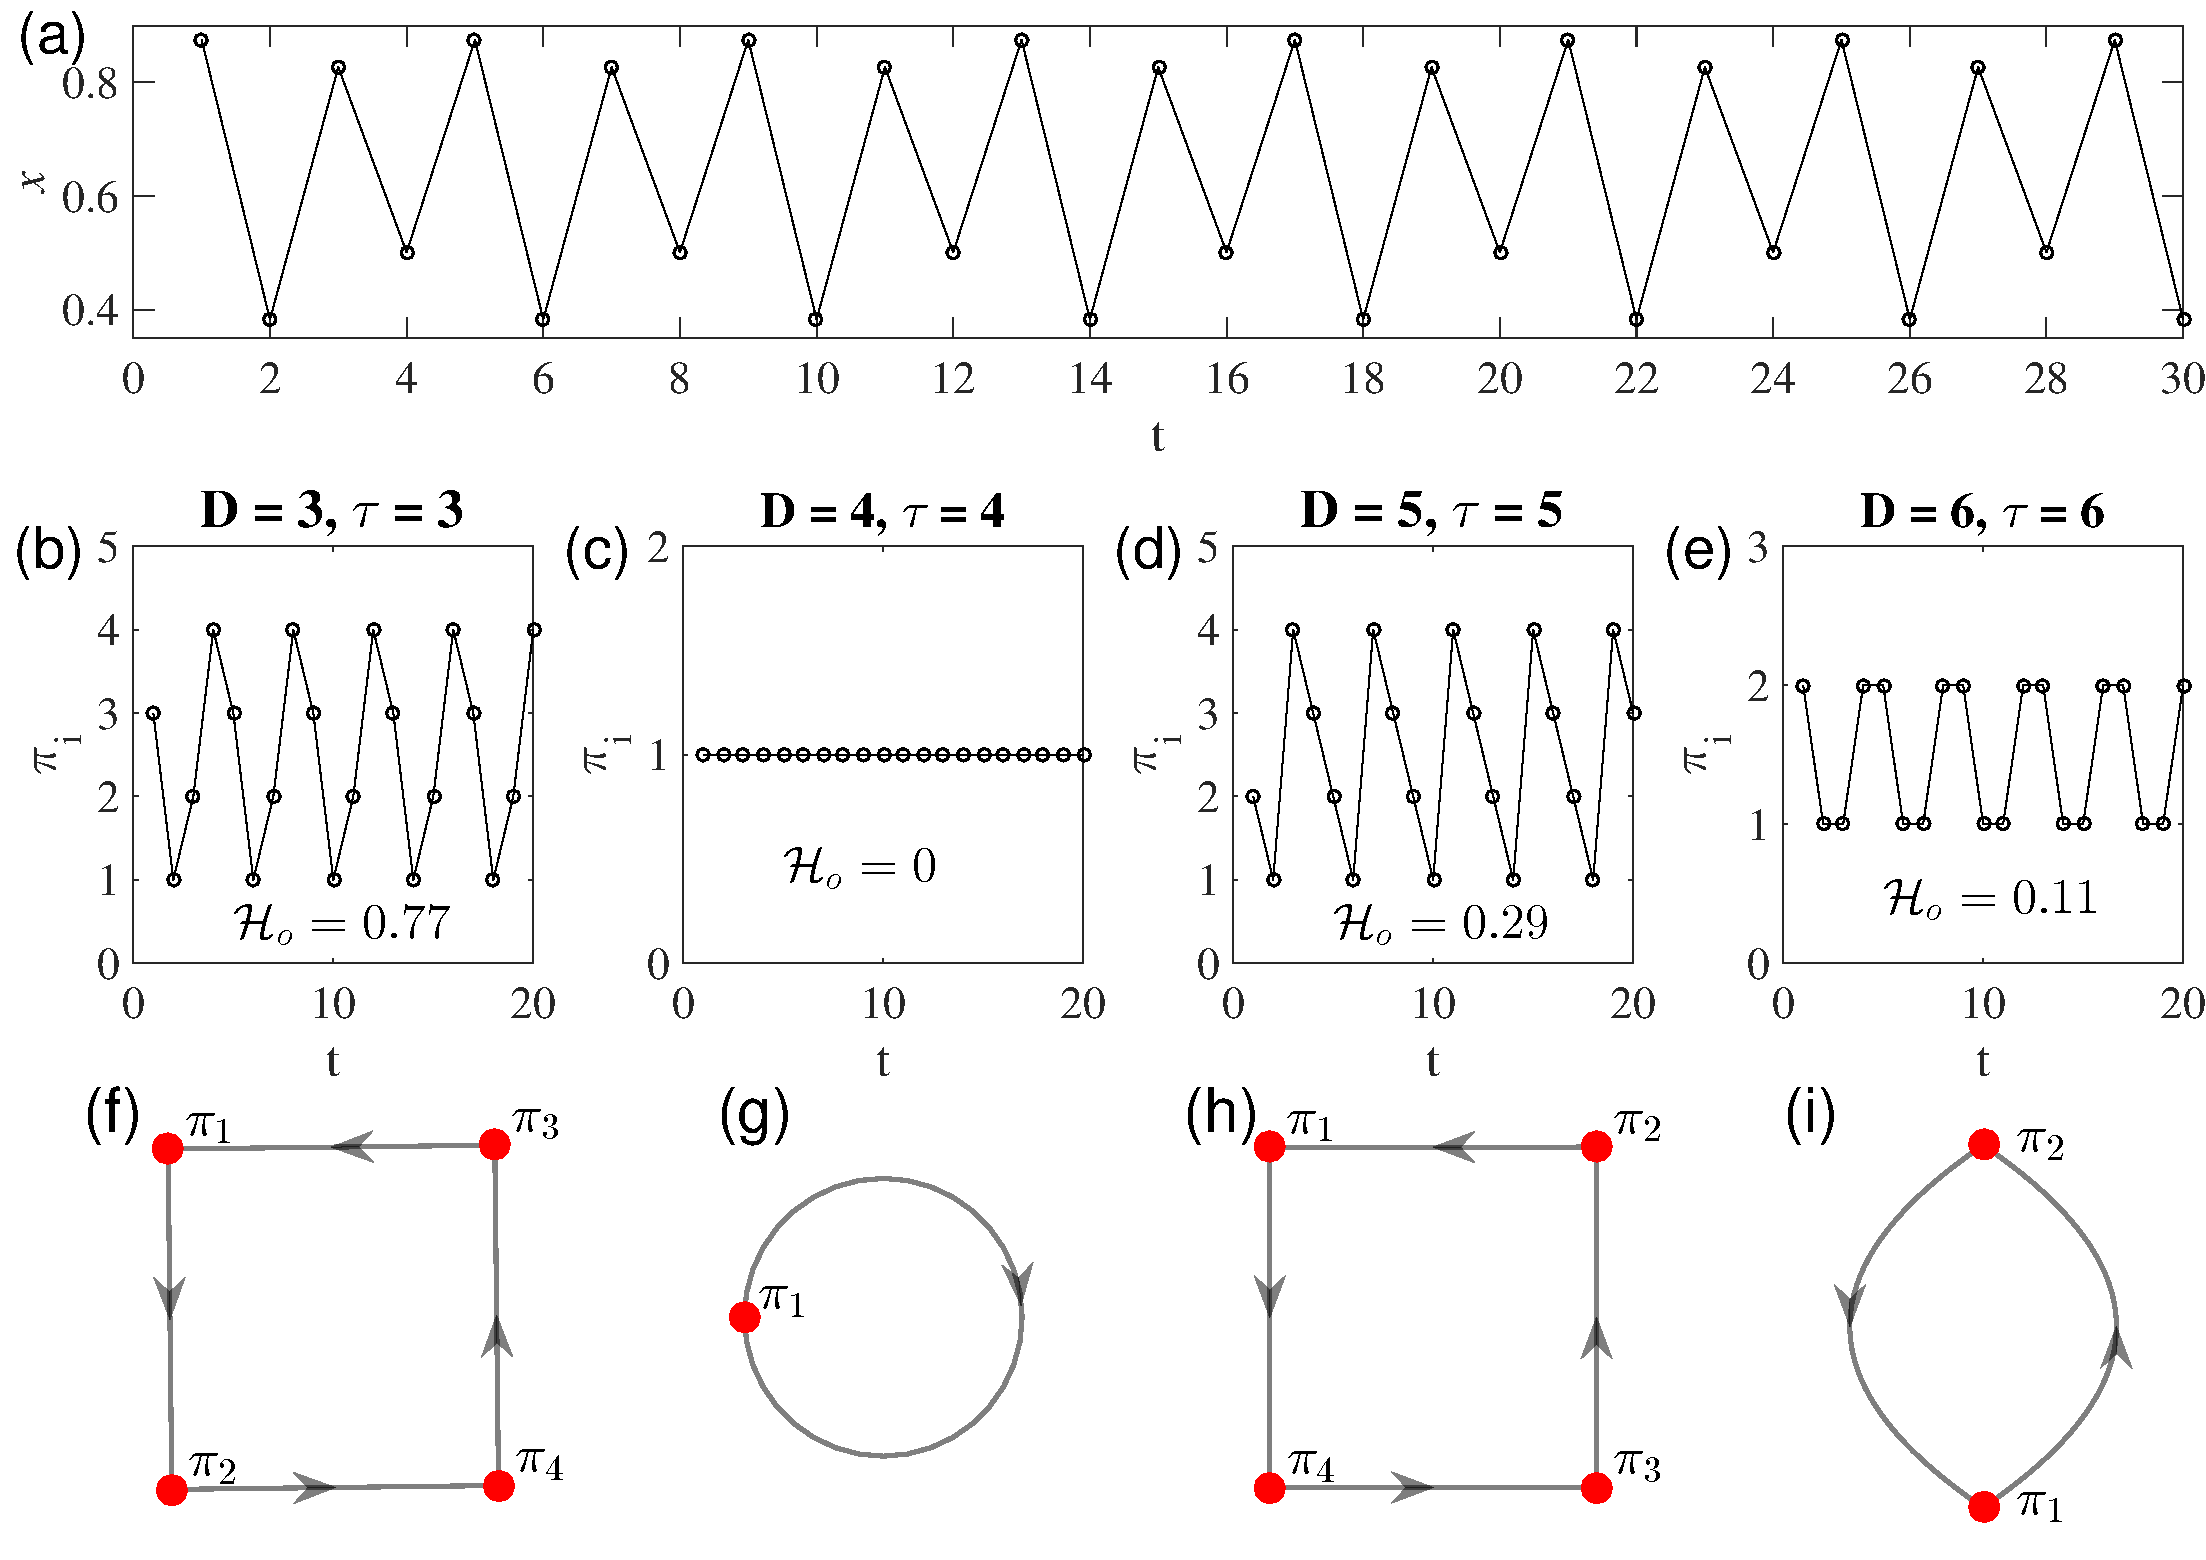
\includegraphics[width=2\columnwidth]{period4_logisticExample.pdf}
\caption{\small{Example of a period-4 time series demonstrating the effects of different choices of the embedding parameters $D$ and $\tau$. (a) Time series comprising 30 iterations of the period-4 orbit. The corresponding ordinal pattern series are shown for different combinations of $D$ and $\tau$: (b) $D = \tau = 3$, (c) $D = \tau = 4$, (d) $D = \tau = 5$, and (e) $D = \tau = 6$. The respective permutation entropy values normalized by $\log D!$ as in Eq.~\eqref{eq:Ho} are indicated in the insets of each panel. Panels (f)-(i) show the corresponding OPTNs. The weights of directed edges are not shown (recall that two slightly different normalizations are considered in this work). Note that in panel (g), there exist exclusively self-loops since $D = \tau = 4$ results in a unique, constant pattern. Missing patterns are suppressed.}
\label{fig:embed}}
\end{figure*}

As an illustrative example highlighting the important roles of $D$ and $\tau$ for ordinal pattern based analysis, we consider a period-4 solution of the logistic map 
\begin{equation}
x_{i+1}=rx_i(1-x_i) 
\end{equation}
\noindent
with $r= 3.5$. For the sake of simplicity, we choose $D = \tau $. In this case, Fig.~\ref{fig:embed} demonstrates that the resulting ordinal pattern sequences are significantly affected by the different parameter settings, which further result in different permutation entropy values $\mathcal{H}_O$. For instance, only one unique ordinal pattern is observed when $D = \tau = 4$ (Fig.~\ref{fig:embed}(c,g)) resulting in $\mathcal{H}_O = 0$, which is due to the coverage of exactly one full period by the particular embedding parameters. Other values of $D$ and $\tau$ however yield non-zero entropy values. The results of Fig.~\ref{fig:embed} may raise concern since different choices if $D$ and $\tau$ will change the placement of the system in the complexity--entropy plane. In the special case of the logistic map, we do not have a unique choice of $D$ and $\tau$ for periodic windows when the control parameter $r$ is varied. In such cases, we should focus more on the transitions between different dynamic regimes. In the following, we will show that the results are robust when the control parameter is systematically changed while keeping the same parameter settings of $D$ and $\tau$.

\subsection{Results for four typical dynamic regimes} \label{sec:four}

We further illustrate the potential of the proposed SCMs to characterize different dynamical regimes and transitions for the logistic map with the control parameter $r$ varying in the range $[3.5, 4]$ with a step size of $\Delta r = 0.001$. In this range of $r$, various dynamical regimes and transitions between them can be found, for instance, period doublings, band merging points, inner and outer crises, and intermittency \cite{Kantz97}, which has made this system serving as a paradigmatic model for assessing nonlinear time series analysis methods \cite{MarwanPLA2009}. 

As a first step, we consider four representative regimes that can be observed at particular values of the control parameter $r$, corresponding to either periodic dynamics or chaotic dynamics close to band merging, in some laminar state, and at the outer crisis. In all examples, we will consistently use the embedding parameters $D = \tau = 6$. In general, we emphasize that a higher value of $D$ leads to a larger variety of ordinal patterns and, hence, a more robust statistics. On the other hand, for evaluating the statistical properties of either pattern frequencies or transition frequencies, this comes on the cost of requiring increasingly longer time series. In the following, we will use realizations of the logistic map comprising $L = 1 \times 10^6$ iterations. 

For all four situations, we investigate the SCMs along with their dual entropy characteristics in detail and summarize the obtained results in Tab.~\ref{tableLog}. We note that several types of chaos--chaos transitions will be discussed in the following: the band merging crisis corresponds to intermittency, the inner crisis to certain chaos-chaos transition and the outer crisis to fully chaotic dynamics. 

\begin{table}[htb]
    {\begin{tabular}{l  l  l  l  l  l  l  l}
    \hline
    Regime & $r$      & $\mathcal{H}_O$ & $\mathcal{C}_O$ & $\mathcal{H}_W$ & $\mathcal{C}_W$ & $\mathcal{H}_E$   & $\mathcal{C}_E$  \\
    \hline
    period-3      & 3.83 & 0 & 0 & 0 & 0 & 0 & 0 \\
    \hline
    band merging    & 3.679 & 0.978 & 0.043 & 0.595 & 0.577 & 0.211 & 0.205  \\
    \hline
    laminar state    & 3.791 & 0.986 & 0.029 & 0.633 & 0.609 & 0.280 & 0.269 \\
    \hline
    outer crisis  & 4.0 & 0.994 & 0.014 & 0.677 & 0.638 & 0.359 & 0.339 \\
    \hline
    \end{tabular}}
   \caption{Statistical complexity measures for four different values of the control parameter $r$ of the logistic map (embedding parameters: $D = \tau = 6$).   \label{tableLog}}    
\end{table}

Due to our choice of $\tau$ and $D$, all SCMs take values of zero for the period-3 series because the temporal distance between each pair of components of the embedding vector covers a multiple of two full periods (cf.~Fig.~\ref{fig:embed}). Other choices of $D$ and $\tau$ would commonly yields non-zero values for the period-3 regime. For the three other cases of band merging, laminar state and outer crisis, the values of all SCMs significantly differ from zero. The pattern frequency based SCM $\mathcal{C}_O$ shows smaller values than the other two measures for all regimes, which implies a positioning in the lower right parts of the complexity--entropy planes in Fig.~\ref{fig:CElogistic}(a). However, for the transition matrix based SCMs, both the estimated entropies $\mathcal{H}_W$, $\mathcal{H}_E$ and associated complexity measures $\mathcal{C}_W$, $\mathcal{C}_E$ show results that are more consistent with the expectations when considering the respective level of chaoticity of the system in those three regimes (i.e., a rising Lyapunov exponent with increasing $r$ in the respective chaotic regimes). In particular, the estimated SCMs take their largest values for $r = 4$ in the outer crisis regime, and the SCMs are the smallest when $r = 3.679$ in the band merging case, while the laminar regime displays intermediate SCM values. 

\subsection{Complexity--entropy planes} \label{sec:plane}

In order to put our previous results into a broader context, we next show the complexity--entropy planes obtained when varying the control parameter $r$ in the logistic map. It is notable that the logistic map has already been widely discussed in the framework of SCMs \cite{RossoPRE2007,MartinPLA2003}, but only for pattern frequency based complexity measures. For each value of $r$, we construct an OPTN from a time series of length $L = 1 \times 10 ^ 6$, after removing the first $1000$ values of transients from the data series. We have repeated the following calculations for embedding parameters $D = \tau \in [2, 7]$. 

When only one unique ordinal pattern is identified in a given time series, all SCMs take a value of $0$, which is reasonable since only self-loops are observed. This however happens only if $D$ is an integer multiple of the period for the periodic windows of the logistic map (e.g., Fig.~\ref{fig:embed}(g)). Another practical concern is the data requirements for computing entropies and complexity measures. For a reliable estimation of SCMs, a pragmatic condition on the length $L$ of the time series $L$ as being sufficiently larger than $D!$ \cite{rossoPRL2007,kowalskiPhyD2007} has been satisfied in our setting for $D \leq 7$. In the particular example of logistic map, one may easily generate realizations of longer lengths, which however do not improve the obtained estimates significantly (as we have tested for $L \leq 5 \times 10^6$, not shown). 

In previous works, SCMs have been applied to distinguish chaos from noise by employing the concept of complexity--entropy plane~\cite{rossoPRL2007}. Generalizing this idea to our OPTN based SCMs, this plane shows the statistical complexity measures ($\mathcal{C}_O$, $\mathcal{C}_W$ and $\mathcal{C}_E$) as a function of the corresponding normalized entropy values ($\mathcal{H}_O$, $\mathcal{H}_W$ and $\mathcal{H}_E$). The three SCMs characterize both randomness and correlation structures in a time series, which in consequence result in a non-trivial dependence on the associated entropy values. Specifically, chaotic systems present maximal complexity while stochastic systems have lower values of complexity, hence appearing in different regions of the complexity--entropy plane~\cite{rossoPRL2007}. Furthermore, for a given entropy value, the range of possible SCM values is bound by a minimum $\mathcal{C}_{min}$ and a maximum $\mathcal{C}_{max}$. A general algorithm for computing the bounds $\mathcal{C}_{min}$ and $\mathcal{C}_{max}$ has been provided in Ref.~\cite{martinPhyA2006}. 

Figure~\ref{fig:CElogistic} shows the complexity--entropy planes for embedding parameters $D = \tau$ varied between $4$ and $6$. We emphasize that the results are qualitatively similar when $D$ and $\tau$ are varied in the interval $[3, 7]$. Furthermore, it is notable that the values of $\mathcal{C}_{max}$ depend on the embedding dimension $D$ since $D$ determines the number of patterns and pattern transitions which are considered in the definition of SCMs. By contrast, $\mathcal{C}_{min}$ shows less dependence on $D$. 

\begin{figure*}
	\centering 
	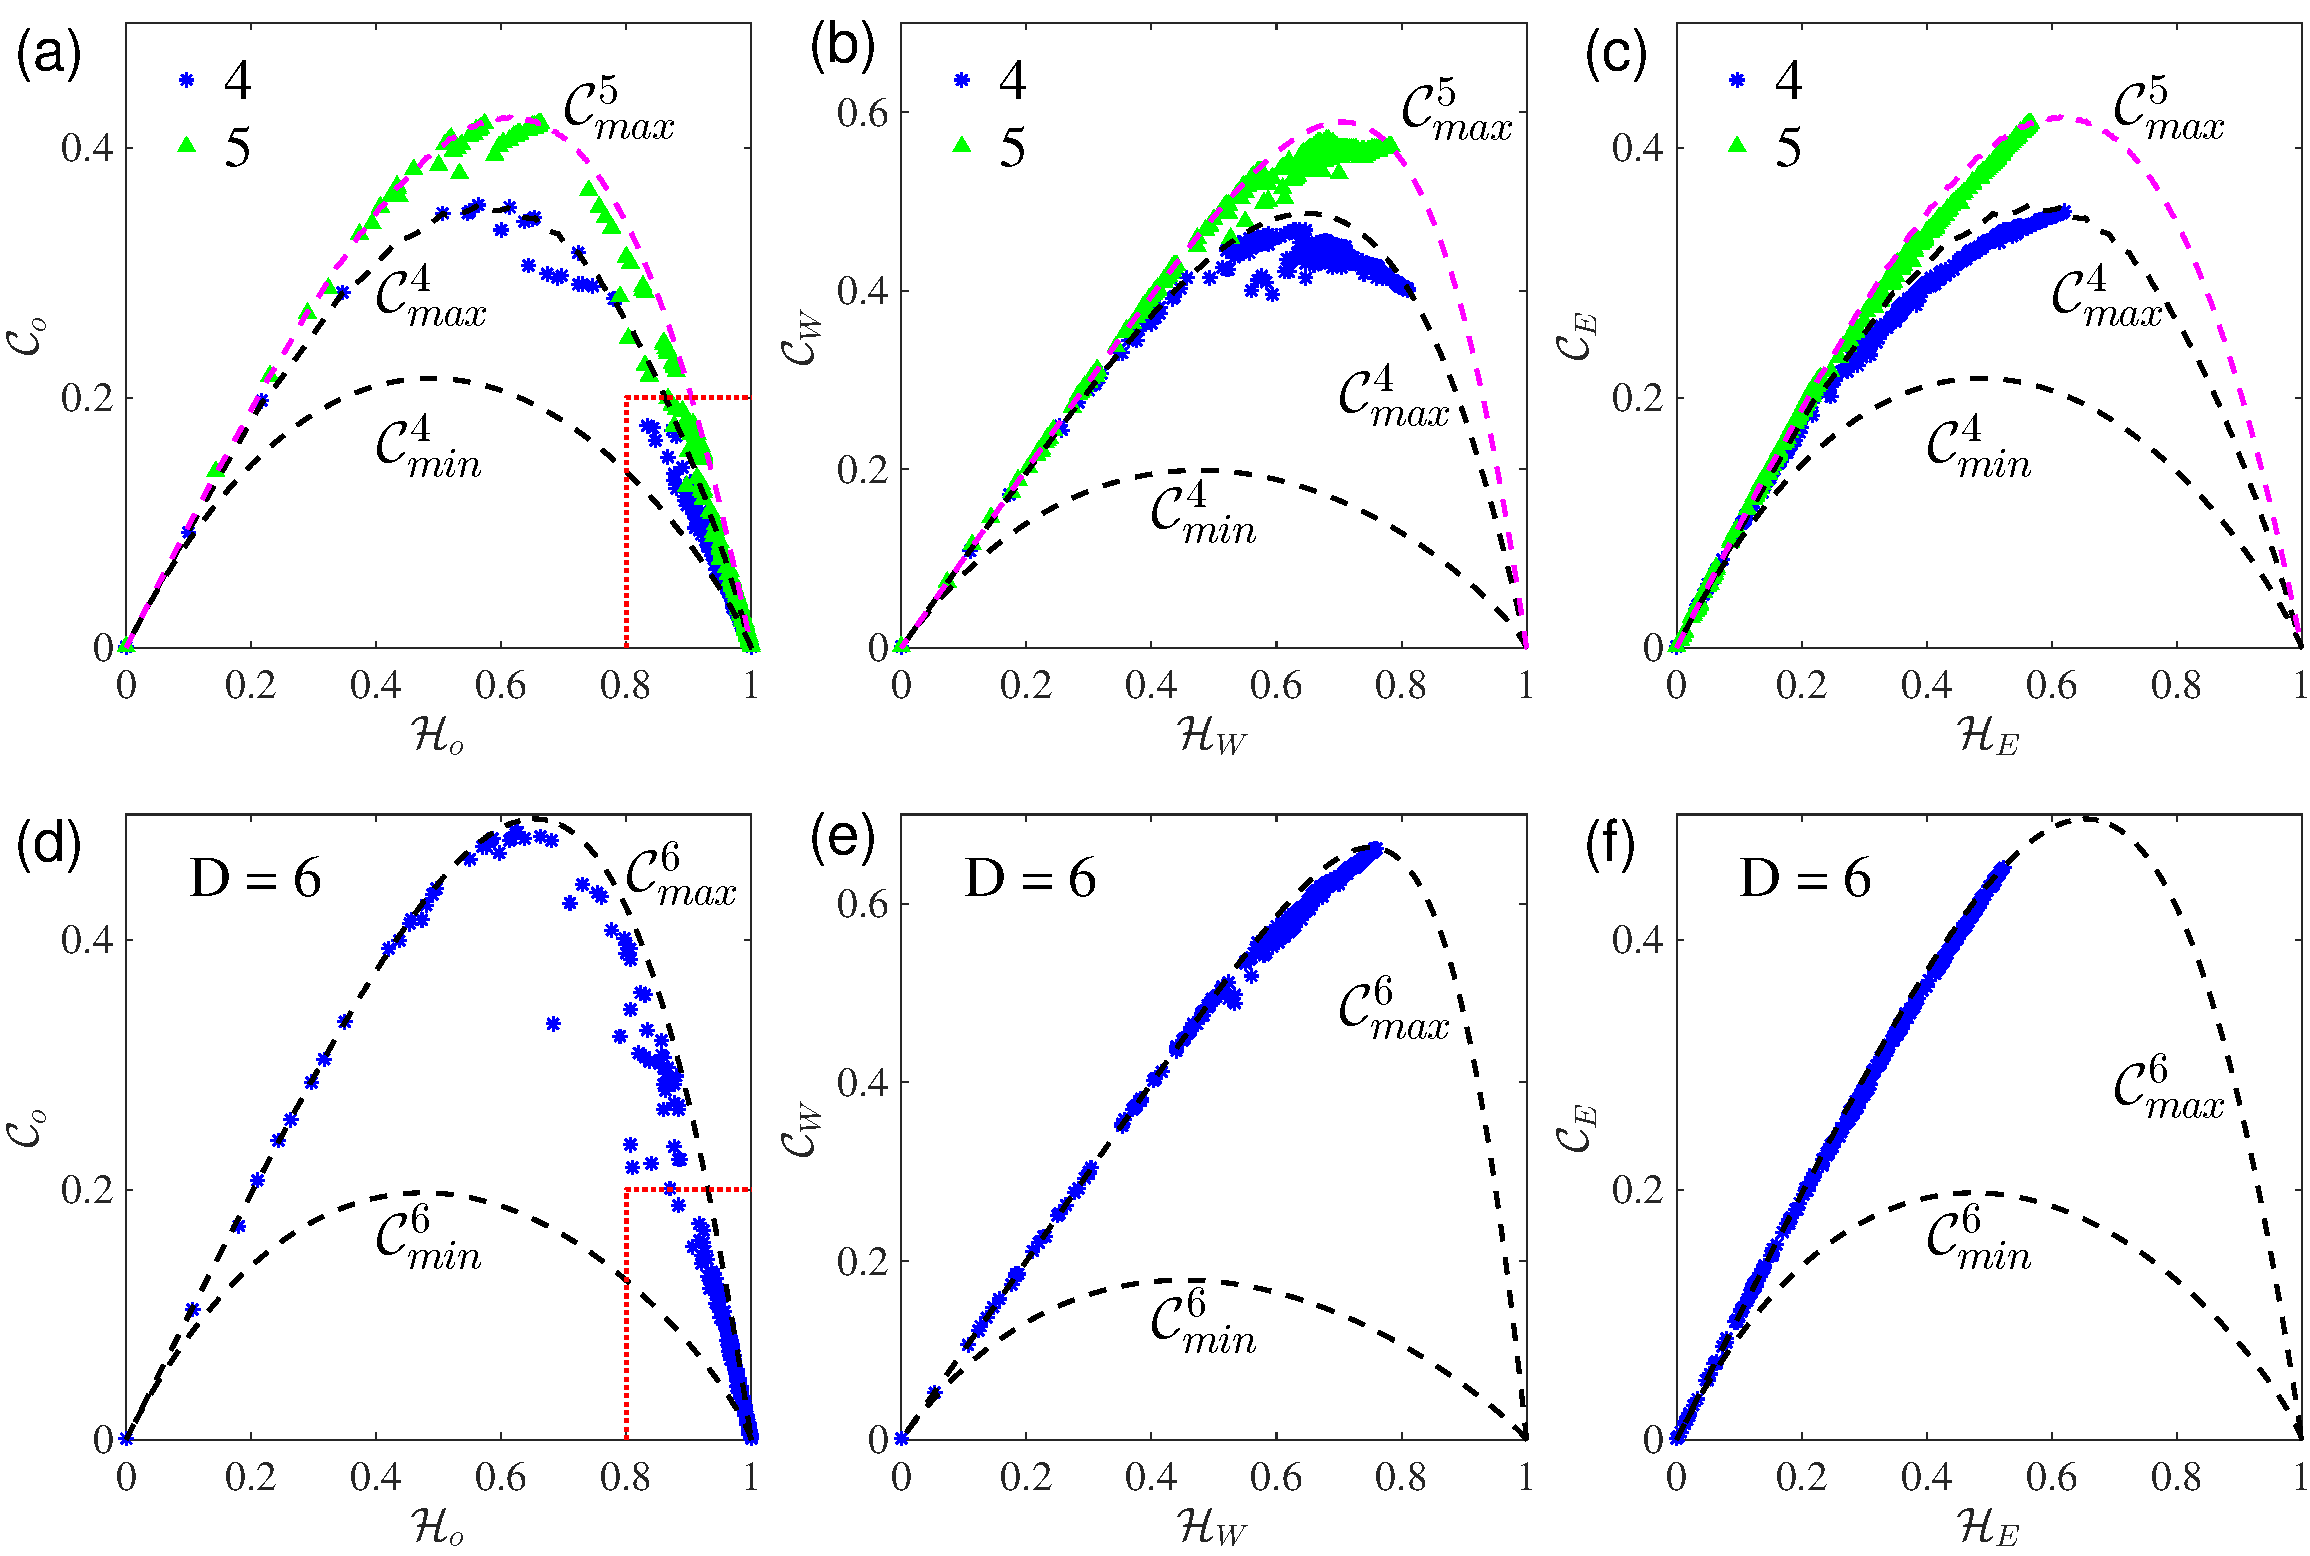
\includegraphics[width=2\columnwidth]{CompEntropy_LogisticHC.pdf}
\caption{\small{(Color online)Three different complexity--entropy planes (based on the Jensen-Shannon divergence) illustrating the behavior of the three SCMs for example series of the logistic map with varying control parameter $r$: (a,d) $\mathcal{C}_O$ versus $\mathcal{H}_O$, (b,e) $\mathcal{C}_{W}$ versus $\mathcal{H}_{W}$, and (c,f) $\mathcal{C}_{E}$ versus $\mathcal{H}_{E}$. The dashed lines correspond to the maximum $\mathcal{C}_{max}$ and minimum complexity $\mathcal{C}_{min}$ values for a fixed value of the entropy. Panels (a-c) show the results for embedding dimensions $D = 4,5$ and (d-f) for $D = 6$. In panels (a,d), the bottom-right rectangles of dotted red lines highlight the regions for the traditional pattern frequency based SCM analysis where the differentiation between stochastic and deterministic--chaotic dynamics is ambiguous. }  \label{fig:CElogistic}}
\end{figure*}

First of all, we recover the known result that pattern frequency based SCM values lie around the maximum curve $\mathcal{C}_{max}$, while the displacements of the estimated values from their theoretical upper bounds depend on the embedding dimension $D$ as shown in Fig.~\ref{fig:CElogistic}(a,d). Most notable, we find many combinations of complexity--entropy values in the lower right part of the plane (high entropy, low complexity), which have been highlighted by rectangles of dotted lines. This region of the plane is challenging for SCMs to distinguish between chaotic time series and random noise~\cite{BorgesAMC2019} and is in our case occupied by values corresponding to chaotic regimes of the logistic map at large $r$ values. The corresponding ambiguity results from the fact that both $\mathcal{H}_O$ and $\mathcal{C}_O$ only take static information in the sense that only pattern frequencies have been considered in their definitions. 

For our new pattern transition based SCMs, we find that in the complexity--entropy planes of $\mathcal{C}_W$ versus $\mathcal{H}_W$ and $\mathcal{C}_E$ versus $\mathcal{H}_E$, the results for the logistic map again closely align with the theoretical upper bounds $\mathcal{C}_{max}$. When increasing the embedding dimension, the estimated values approach the theoretical $\mathcal{C}_{max}$ curve more and more closely and essentially cover the left uprising branch of the curve for the SCM based exclusively on transition frequencies (Fig.~\ref{fig:CElogistic}(b,d)). By contrast, the definition of $\mathcal{C}_{E}$ and $\mathcal{H}_{E}$ takes information on both, pattern frequencies and transition frequencies into account, which results in the obtained SCM values aligning even more closely with $\mathcal{C}_{max}$ already at lower embedding dimensions (Fig.~\ref{fig:CElogistic}(c,f)). The most interesting result is, however, that we do not find any values in the lower right part of the plane, which for the classical SCM based on permutation entropy would present the challenging region of ambiguity. We therefore suggest that it is the deterministic transition behavior among patterns that makes the distinction from random noise. 

Based on the results of Fig.~\ref{fig:CElogistic}, we conclude that the pattern transition behavior encoded in the OPTNs provides novel insights that can be exploited in terms of SCMs that complement their traditional counterparts. 

%% update but not properly integrated 
We compare the results with fractional Brownian motion (fBm), which has long-range temporal correlations \cite{Mandelbrot1968}. Specifically, for an fBm process the long range of the process is characterized by the Hurst exponent $\alpha$ when positively correlated (persistence) for $1/2 < \alpha < 1$, while suppressed (anti-persistence) for $0< \alpha < 1/2$. $\alpha=1/2$ corresponds to the classical Brownian motion. In an analogy to the previous case of Logistic map of varying control parameter $r$, we generate time series for varying $\alpha \in (0, 1)$ with step size 0.05 and the results are shown in Fig. \ref{fig:CEfBm}. 

By the same time, we transform the fBm series into a stationary one by a first-order difference filter, i.e., by considering its increments $x_{i+1}- x_i$. The transformed series is commonly referred to as fractional Gaussian noise (fGn). Notably, fGn retains the long-range correlations and Gaussian probability density function (PDF) from the underlying
fBm process. Note that the time delay embedding issues of both fBm and fGn have been discussed in detail in \cite{Zou2015}. The complexity--entropy planes of fGn are shown in Fig. \ref{fig:CEfGn}. 

First, the traditional pattern frequency based SCMs values are reproduced as shown in the Figures \ref{fig:CEfBm}(a, d) and \ref{fig:CEfGn}(a, d) fGn, which agree with that have been reported in \cite{RossoPRE2007,rossoPRL2007}. 

\begin{figure*}
	\centering 
	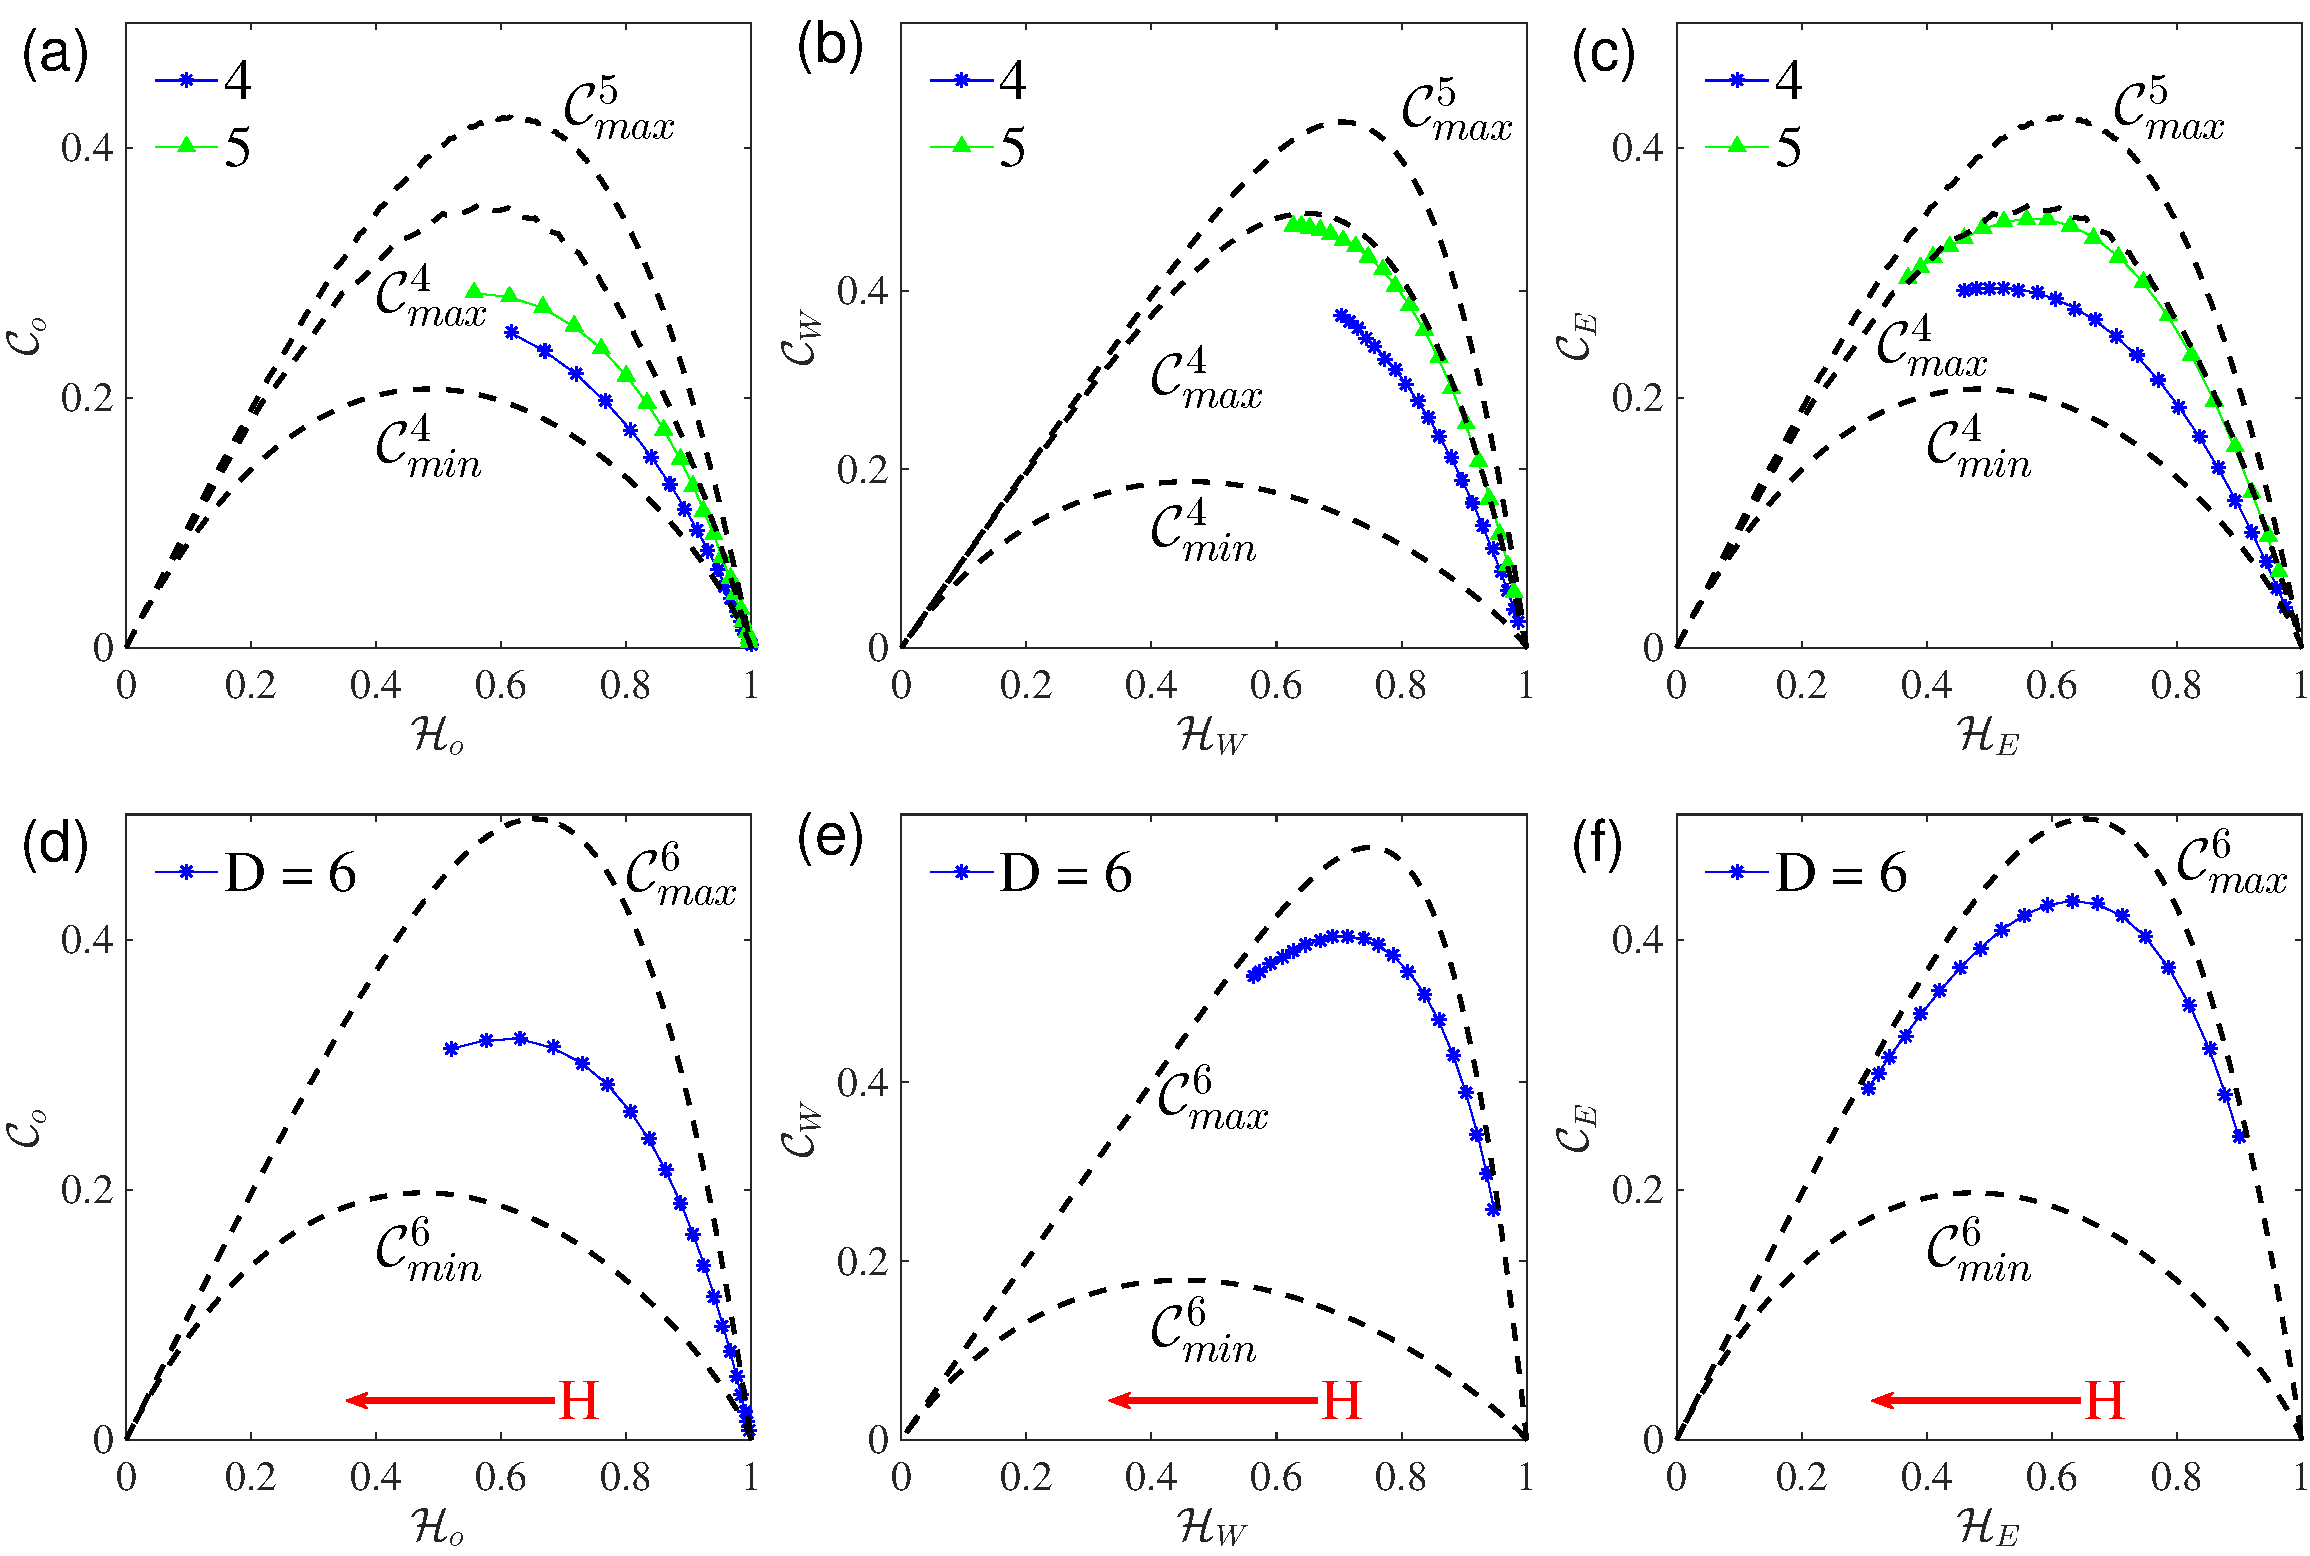
\includegraphics[width=2\columnwidth]{CompEntropy_fBm.pdf}
\caption{\small{(Color online) Similar with Fig. \ref{fig:CElogistic} but for fractional Brownian motion of Hurst exponent $\alpha \in (0, 1)$ with step size 0.05. (a,d) $\mathcal{C}_O$ versus $\mathcal{H}_O$, (b,e) $\mathcal{C}_{W}$ versus $\mathcal{H}_{W}$, and (c,f) $\mathcal{C}_{E}$ versus $\mathcal{H}_{E}$. The dashed lines correspond to the maximum $\mathcal{C}_{max}$ and minimum complexity $\mathcal{C}_{min}$ values for a fixed value of the entropy. Panels (a-c) show the results for embedding dimensions $D = 4,5$ and (d-f) for $D = 6$. }  \label{fig:CEfBm}}
\end{figure*}

\begin{figure*}
	\centering 
	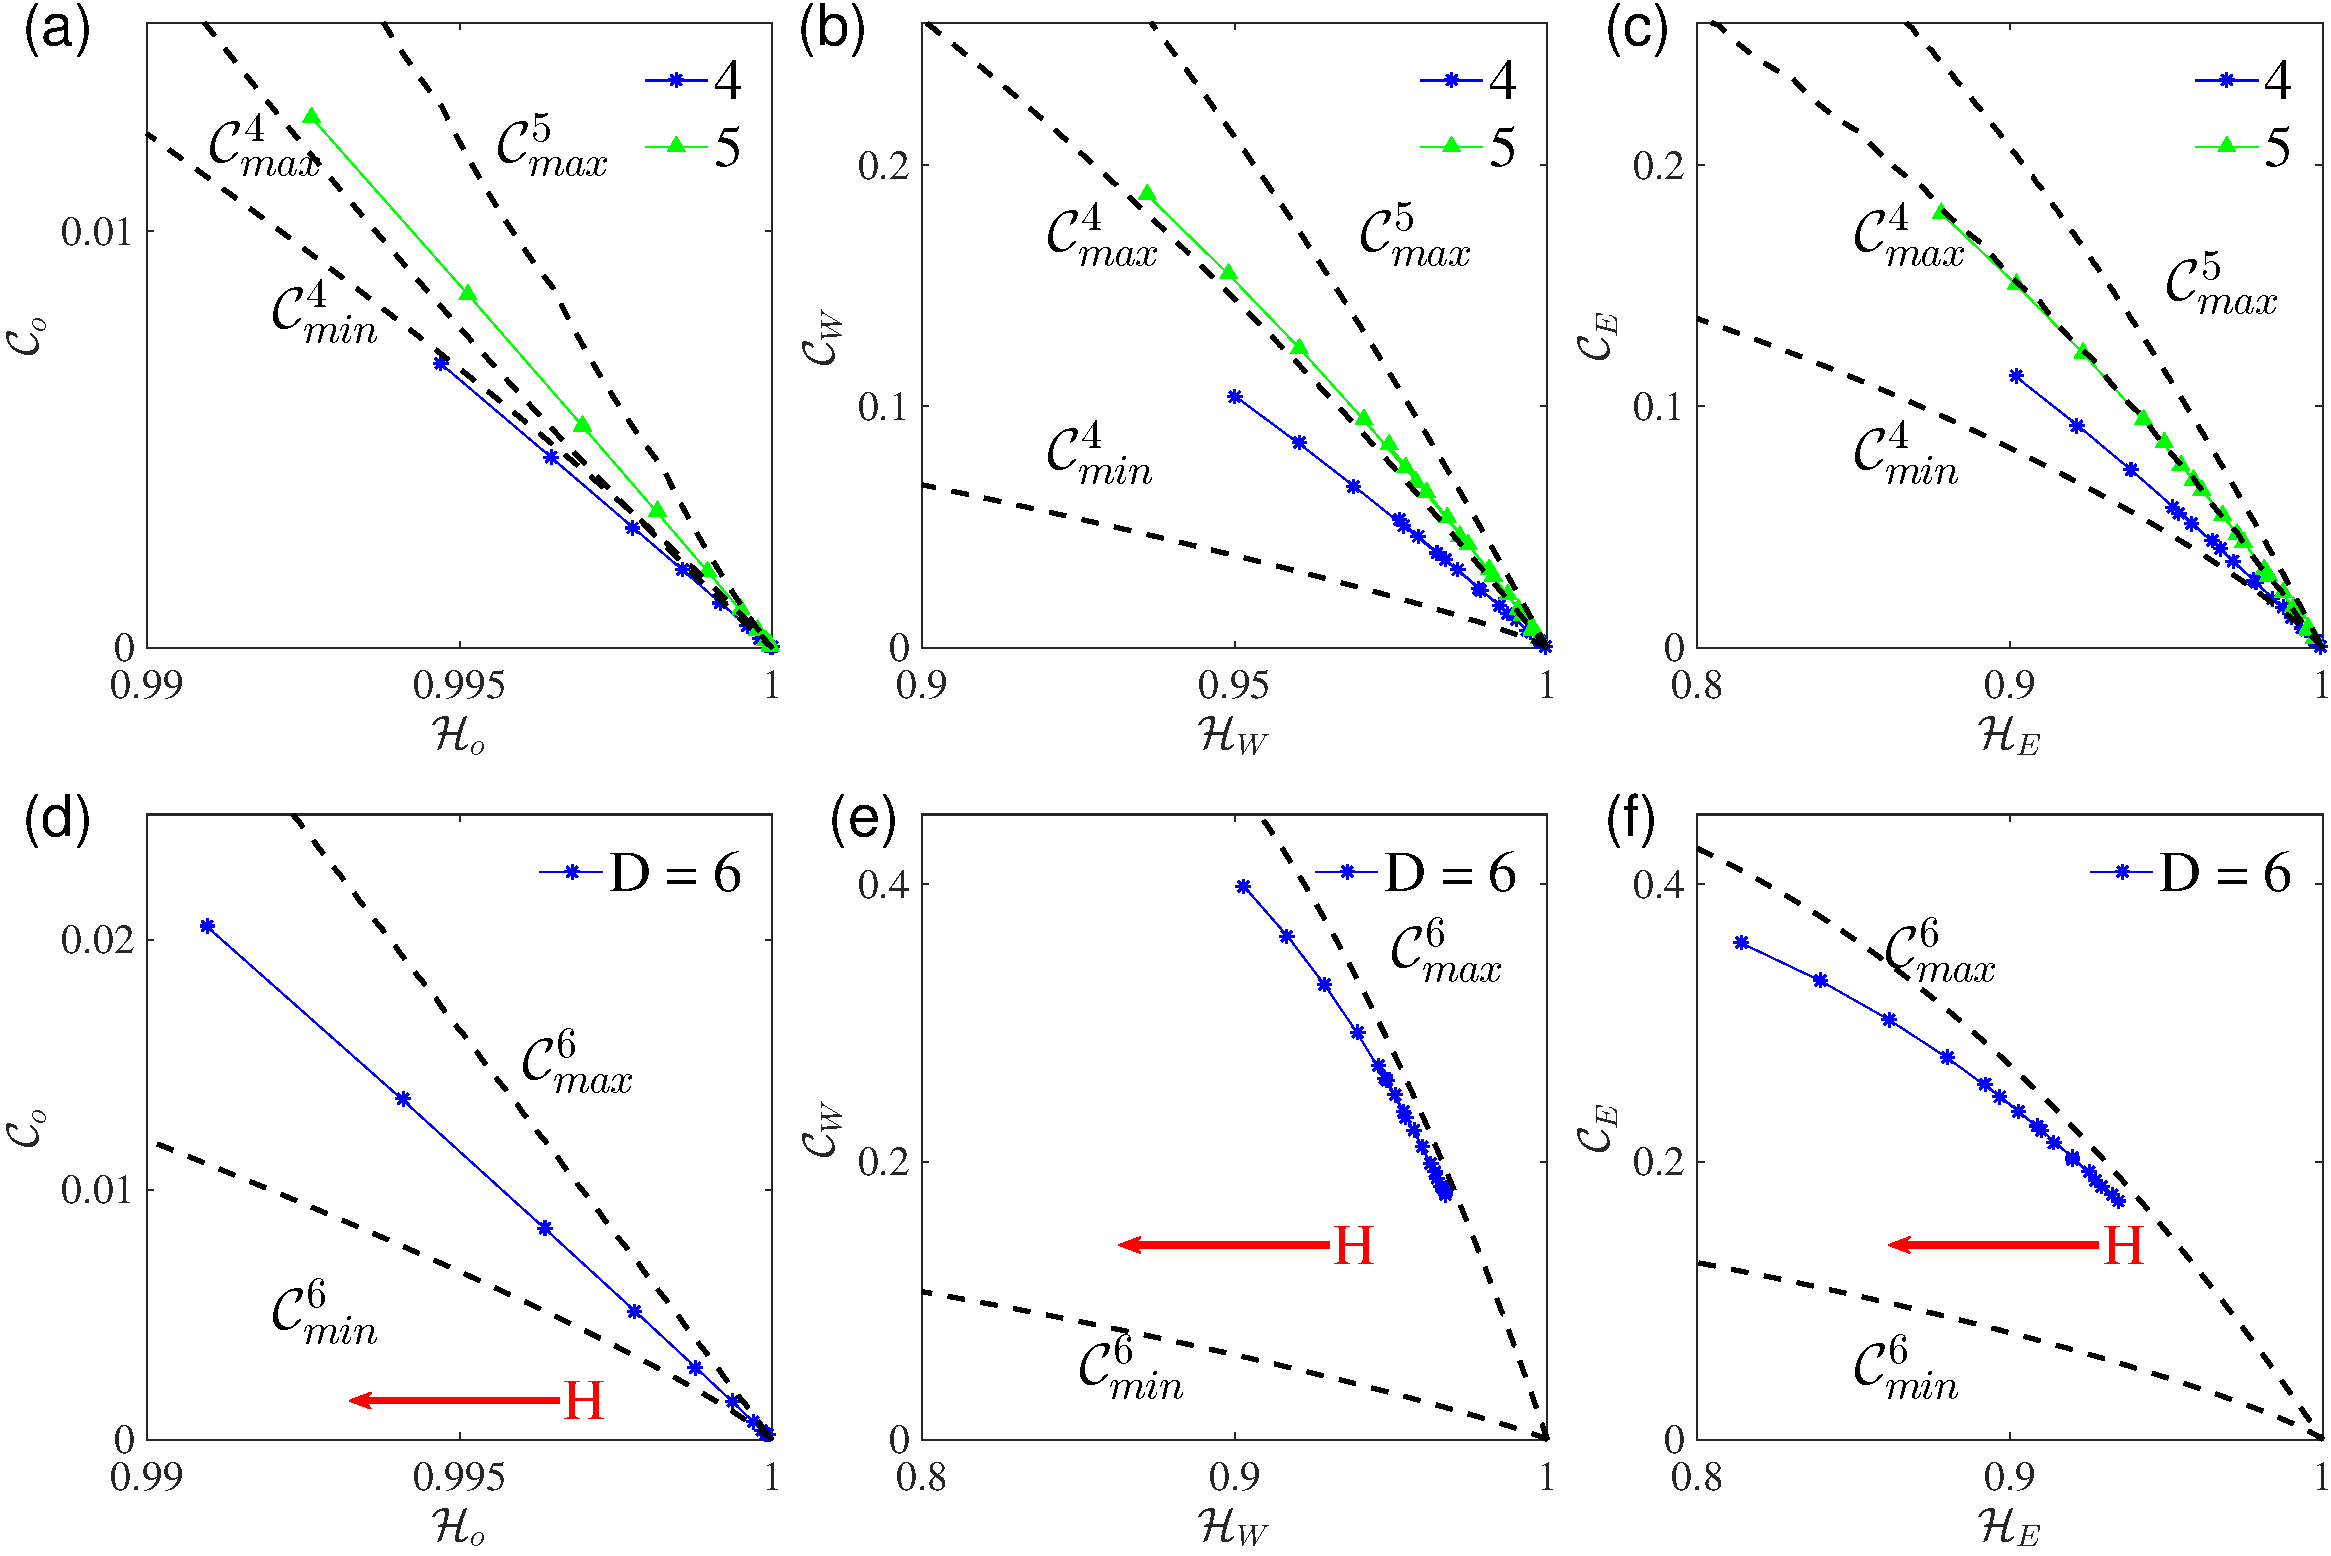
\includegraphics[width=2\columnwidth]{CompEntropy_fGn.pdf}
\caption{\small{(Color online) Similar with Fig. \ref{fig:CElogistic} but for fractional Gaussian noise Hurst exponent $\alpha \in (0, 1)$ with step size 0.05. (a,d) $\mathcal{C}_O$ versus $\mathcal{H}_O$, (b,e) $\mathcal{C}_{W}$ versus $\mathcal{H}_{W}$, and (c,f) $\mathcal{C}_{E}$ versus $\mathcal{H}_{E}$. The dashed lines correspond to the maximum $\mathcal{C}_{max}$ and minimum complexity $\mathcal{C}_{min}$ values for a fixed value of the entropy. Panels (a-c) show the results for embedding dimensions $D = 4,5$ and (d-f) for $D = 6$.  }  \label{fig:CEfGn}}
\end{figure*}


\subsection{Characterizing dynamical transitions} \label{sec:transi}
The logistic map experiences a sequences of different types of bifurcations when the control parameter $r$ is systematically increased. However, the corresponding dynamical regimes and regime transitions are not easy to identify from the complexity--entropy planes discussed above. In the following, we therefore aim to expand the previous results by showing the dependence of our SCMs on the control parameter $r$. Here, our motivation is to verify whether the normalized entropies and associated SCMs computed from OPTNs are indeed able to detect the dynamical transitions along the complex bifurcation scenarios of the logistic map and hence track qualitative changes in the dynamics, including both period--chaos and chaos--chaos transitions. For the sake of comparison, we take the associated Lyapunov exponent of the logistic map as an established measure for characterizing the type of dynamics (regular versus chaotic) along with the degree of chaoticity.

\begin{figure*}
	\centering 
	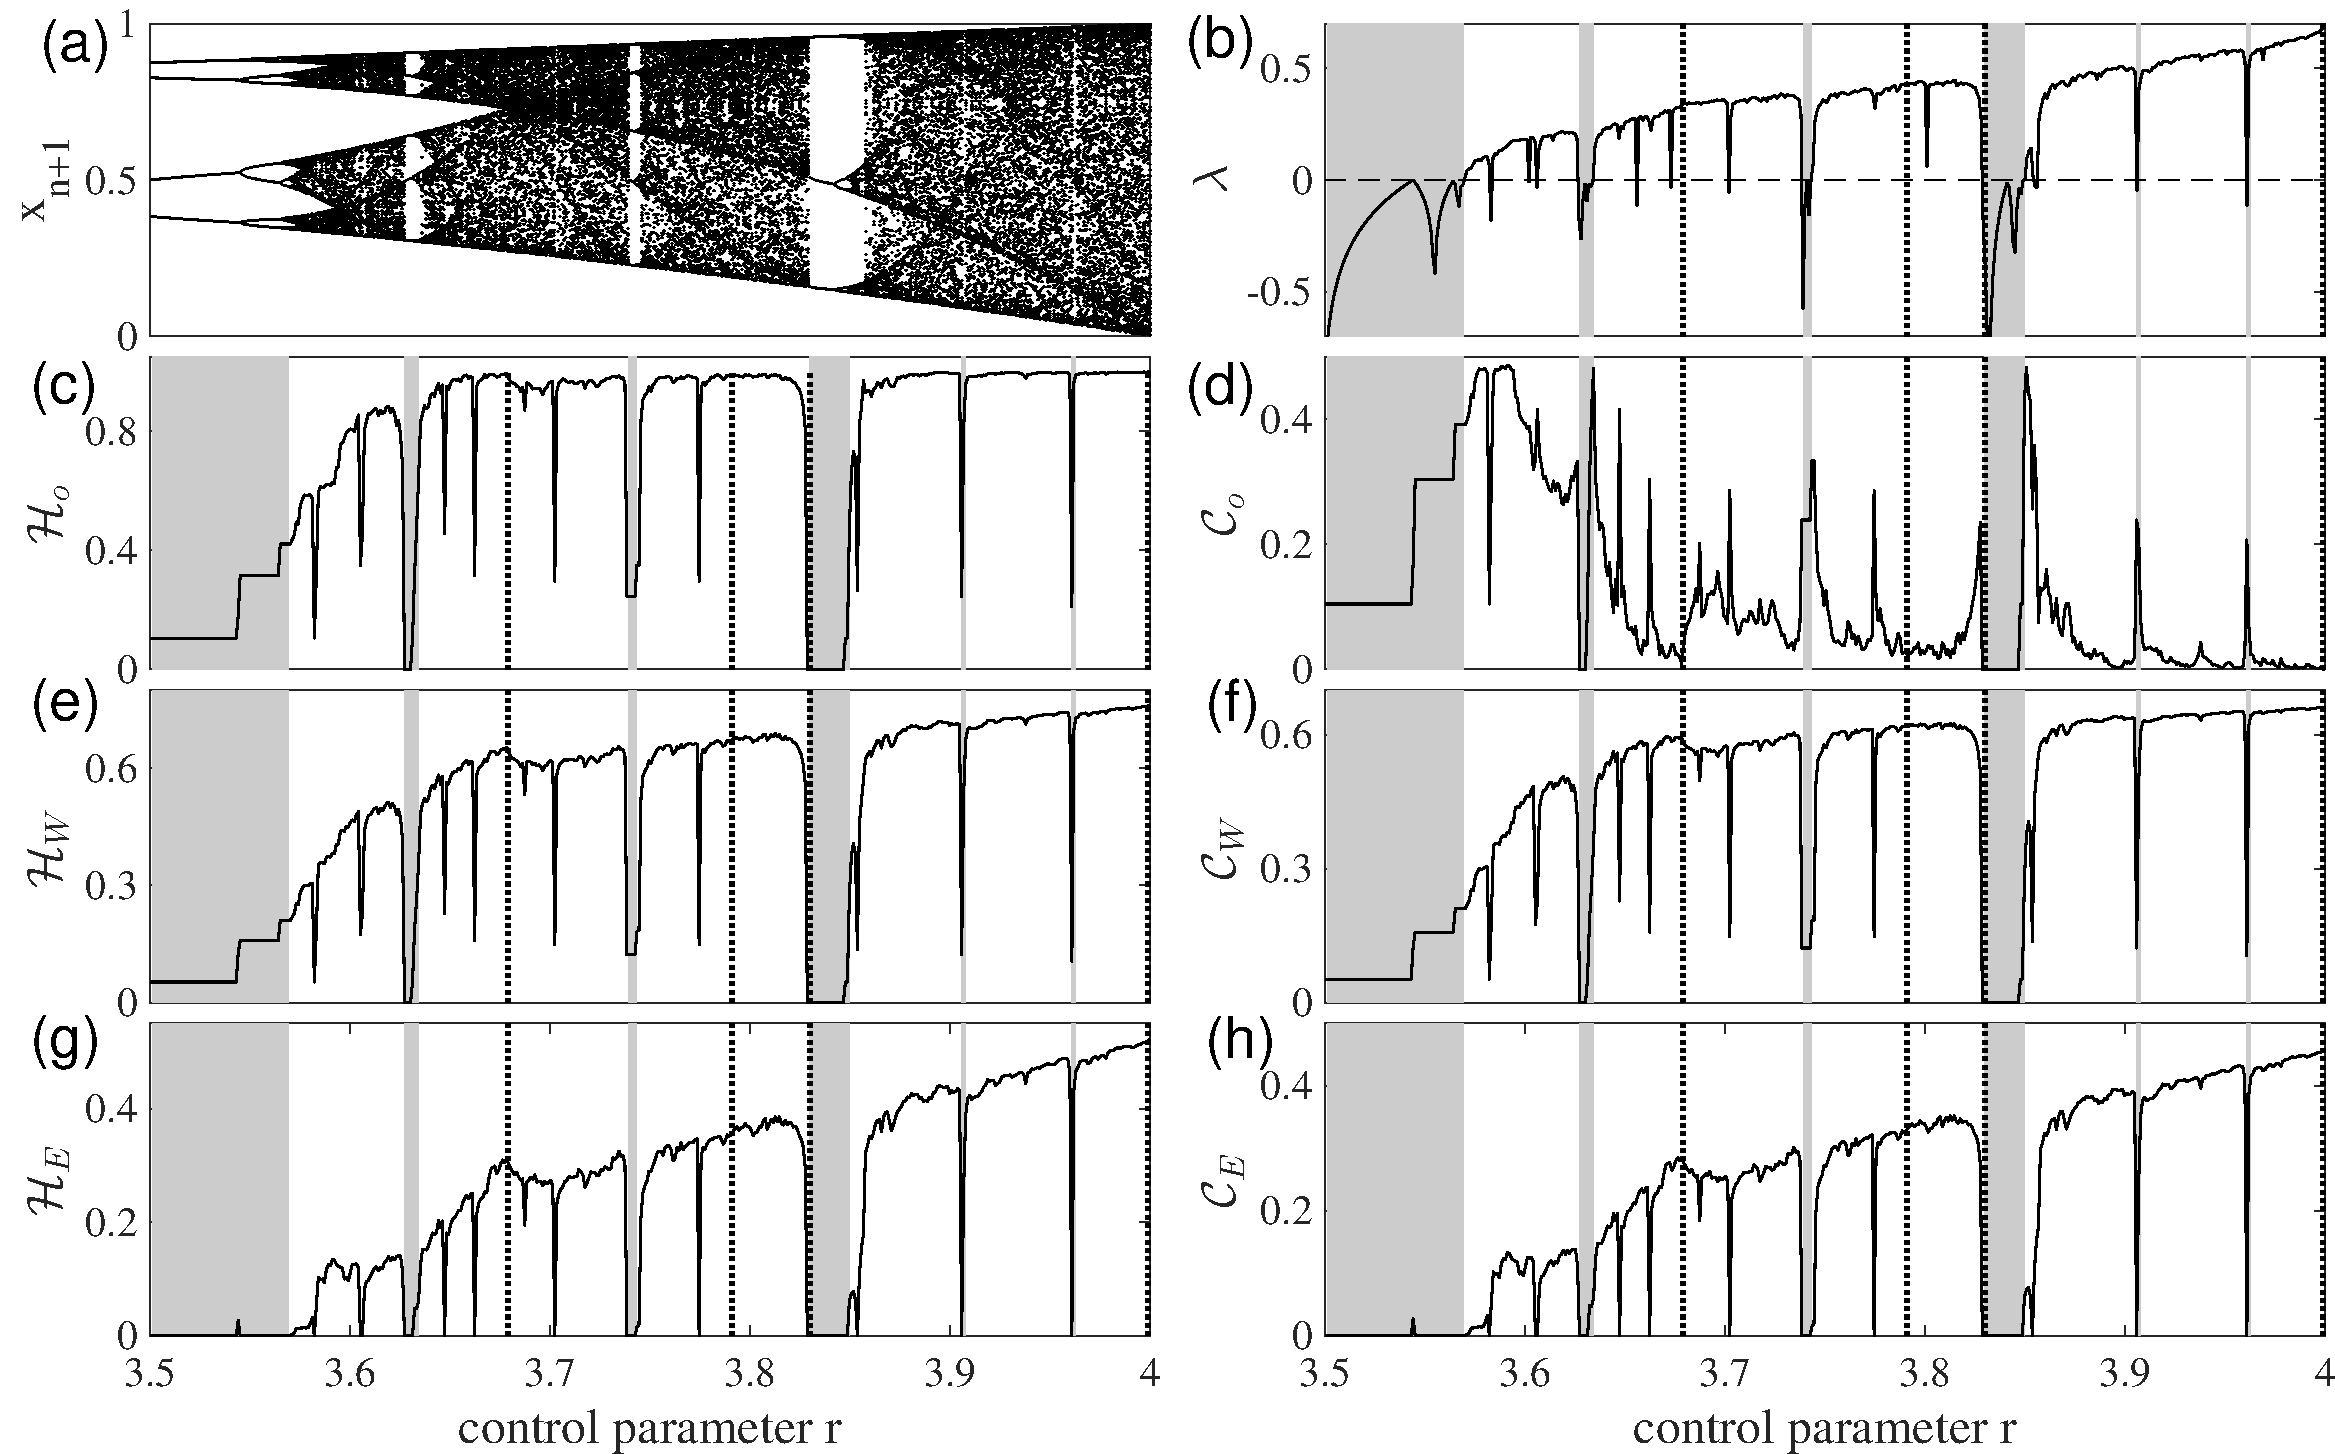
\includegraphics[width=2\columnwidth]{logisticEntropy.pdf}
\caption{\small{Behavior of the different SCMs and associated entropy characteristics for the logistic map in dependence on the control parameter $r$. (a) Bifurcation diagram, (b) Lyapunov exponent, (c) pattern frequency based (permutation) entropy $\mathcal{S}_O$ and (d) associated complexity measure $\mathcal{C}_O$; (e) pattern transition frequency based entropy $\mathcal{S}_W$ based on the globally normalized weight matrix $\mathbf{W}$ and (f) the corresponding complexity measure $\mathcal{C}_W$, and (g,h) entropy $\mathcal{S}_E$ and complexity measure $\mathcal{C}_E$ based on the node-wise out-link normalized weight matrix $\mathbf{W}$. Several major periodic windows have been highlighted by grey background shading. Vertical dotted lines indicate the cases summarized in Tab.~\ref{tableLog}. } \label{fig:bifurcation}}
\end{figure*}

As a general observation, we find that all three SCMs clearly follow the changes in the bifurcation diagram, for instance, showing distinct values in periodic windows (highlighted by grey color in Fig.~\ref{fig:bifurcation}). Other than $\mathcal{C}_O$, the two transition frequency based SCMs behave in a similar way as the Lyapunov exponent. Specifically, as the control parameter $r$ is increased, the chaoticity level grows gradually, reaching a maximum at $r = 4$, which is reflected in an increase in the statistical complexity. A similar increase is absent in the pattern frequency based complexity measure $\mathcal{C}_O$ (Fig.~\ref{fig:bifurcation}(c)). In this context, we note that it is an established fact that pattern frequency based SCMs often do not trace the growth in the chaoticity of the logistic map~\cite{MartinPLA2003}, which can however be improved by using Wooter's distance function instead of the Shannon-Jensen divergence used in this work. From this point of view, the pattern transition frequency based SCMs $\mathcal{C}_W$ and $\mathcal{C}_E$ exhibit more informative behavior in the sense that they track the growth of the level of chaoticity. 

Another conceptual improvement is found for $\mathcal{H}_E$ and $\mathcal{C}_E$ in the parameter range where the logistic map presents period doubling bifurcations, for example, at $r = 3.544$ (Fig.~\ref{fig:bifurcation}(g,h)). It may be noticed that $\mathcal{H}_O$, $\mathcal{C}_O$, $\mathcal{H}_W$ and $\mathcal{C}_W$ all exhibit non-zero values in this parameter range despite a purely periodic dynamics. Furthermore, there are jumps of all four measures at the points of period doubling bifurcations, which have been also reported earlier in Ref.~\cite{BandtPRL2002}. These jumps however are not desirable since the complexity of the dynamics does not change when $r$ passes any of those points. For the case of the period doubling bifurcation at $r=3.544$ (replacing a period-4 by a period-8 solution), we show in Fig.~\ref{fig:transient} that the observed jump in the entropy and SCM values may be explained by accumulated numerical errors during the iterations attracted to the periodic-4 points, which yields long transients. \textcolor{red}{I do not fully get this reasoning...} For estimations based on time series of finite length as used in this work, $\mathcal{H}_E$ and $\mathcal{C}_E$ are however not affected in the same way. Certainly, we should not over-interpret their capabilities since numerical inaccuracy would be accumulated in a longer iterative process such that different ordinal patterns are identified. In addition, there are many periodic windows of different periods along the axis of control parameter $r$, which prevents us from using a unique predefined number of iterations as initial transients for time series of different period length. Notably, similar jumps have also been observed when the system bifurcates from a period-3 to a period-6 solution at $r = 3.842$. 

\begin{figure}
	\centering
	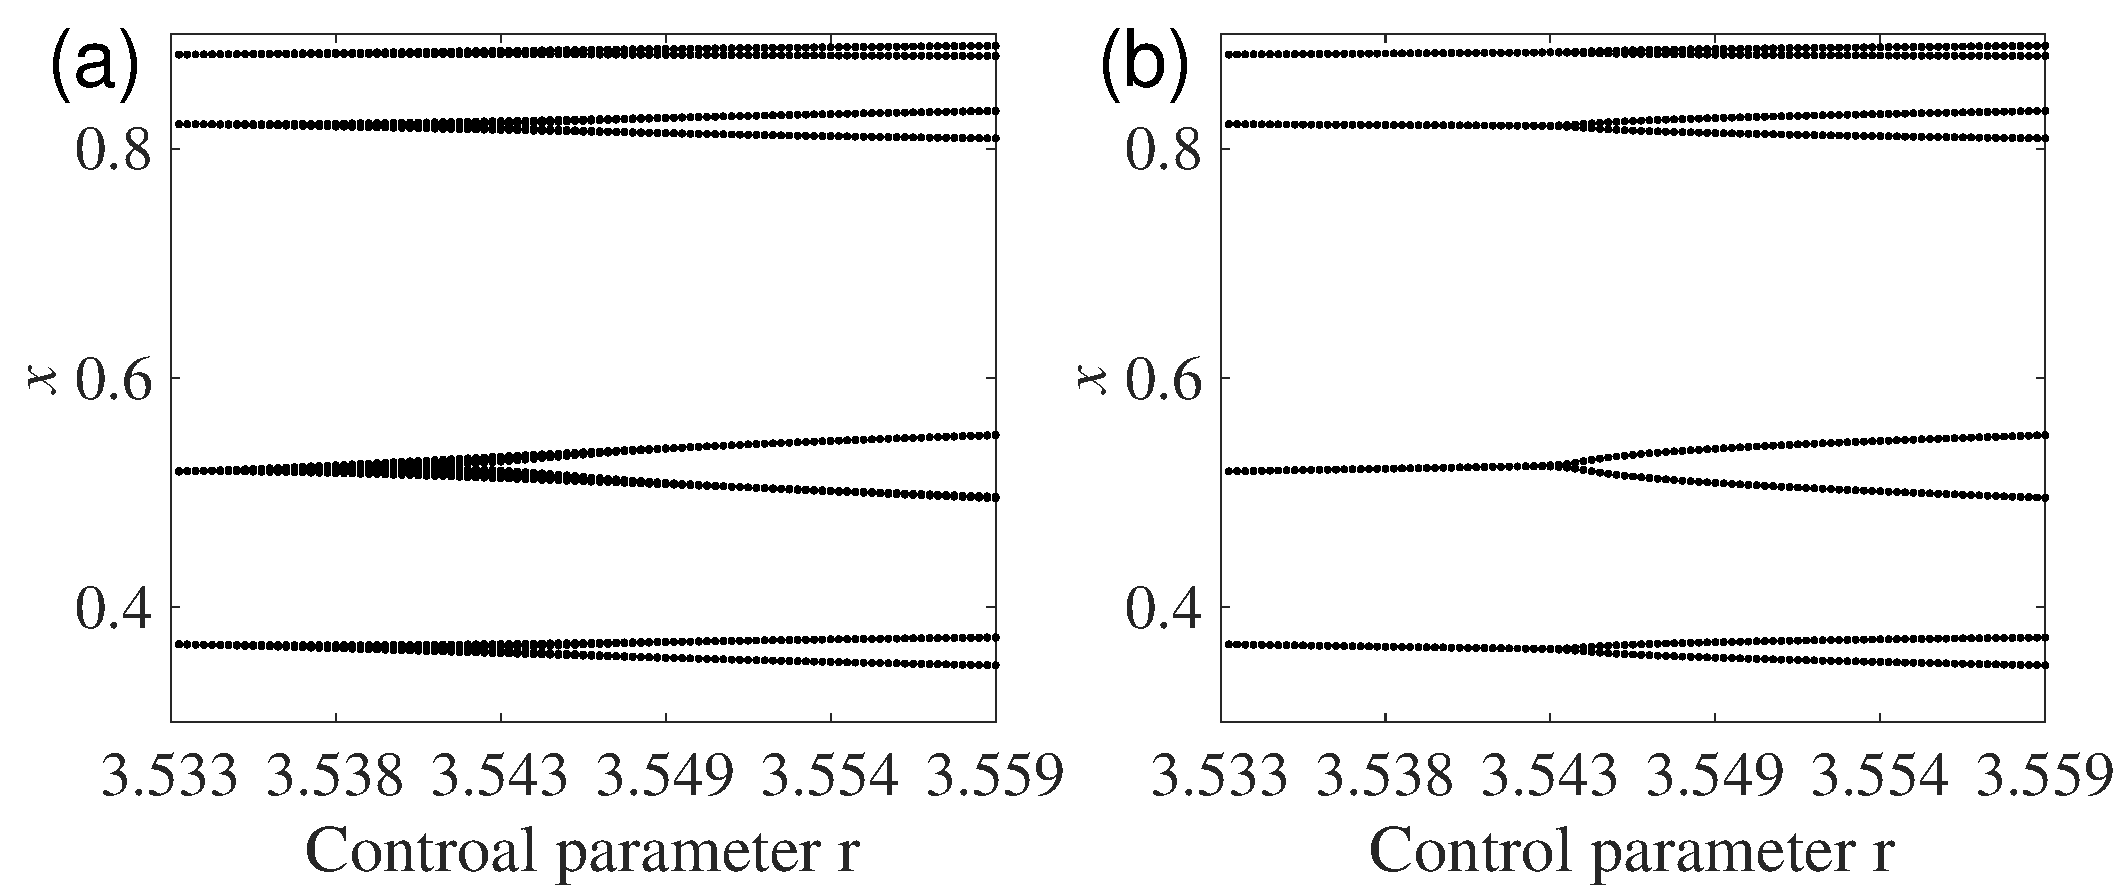
\includegraphics[width=\columnwidth]{period4_exampleTransients.pdf}
\caption{\small{Transient effects in the generation of proper bifurcation diagrams for the logistic map, exemplified by the period doubling bifurcation from a period-4 to a period-8 solution. (a) The actual bifurcation point gets blurred when $r$ is close to $3.544$ if only a short transient of $50$ iterations is removed from the time series. (b) A large number of initial iterations ($2000$) are removed, the correct bifurcation point becomes visible. }\label{fig:transient}}
\end{figure}

\subsection{Dynamical transitions in continuous system}\label{sec:cont}

While we have focused exclusively on the case of the time-discrete logistic map so far, it may be interesting to identify whether a similar behavior can also be obtained for time-continuous deterministic dynamical systems. To this end, we will illustrate a corresponding analysis for the example of the chaotic R\"ossler system \cite{Roessler1976} 
\begin{eqnarray}
\dot{x} &=& -y-z, \nonumber \\
\dot{y} &=& x+0.2y, \\
\dot{z} &=& b+z(x-5.7) \nonumber
\end{eqnarray}
while varying the control parameter $b$. From a conceptual perspective, constructing OPTNs for time series from continuous systems faces certain additional practical challenges, including the proper choice of sampling frequency and embedding parameters, which depend on the particular time scales of the system. To avoid any corresponding discussion on proper choices of further algorithmic parameters, we employ here a Poincar\'e section to each sample trajectory of the system at $y=0$, $\dot{y}<0$ (for different values of $b$) and construct OPTNs from $N = 10,000$ intersection points. The results are shown in Fig. \ref{fig:bifurRossler}. To this end, we conclude that the general behavior of the different SCMs and associated entropy measures resembles that previously observed for the logistic map in Fig.~\ref{fig:bifurcation}. Specifically, all measures trace the succession of bifurcations in the considered range of $b$. We outline more detailed follow-up investigations on the behavior of our OPTN based SCMs as relevant topics for future work.

\begin{figure*}
	\centering 
	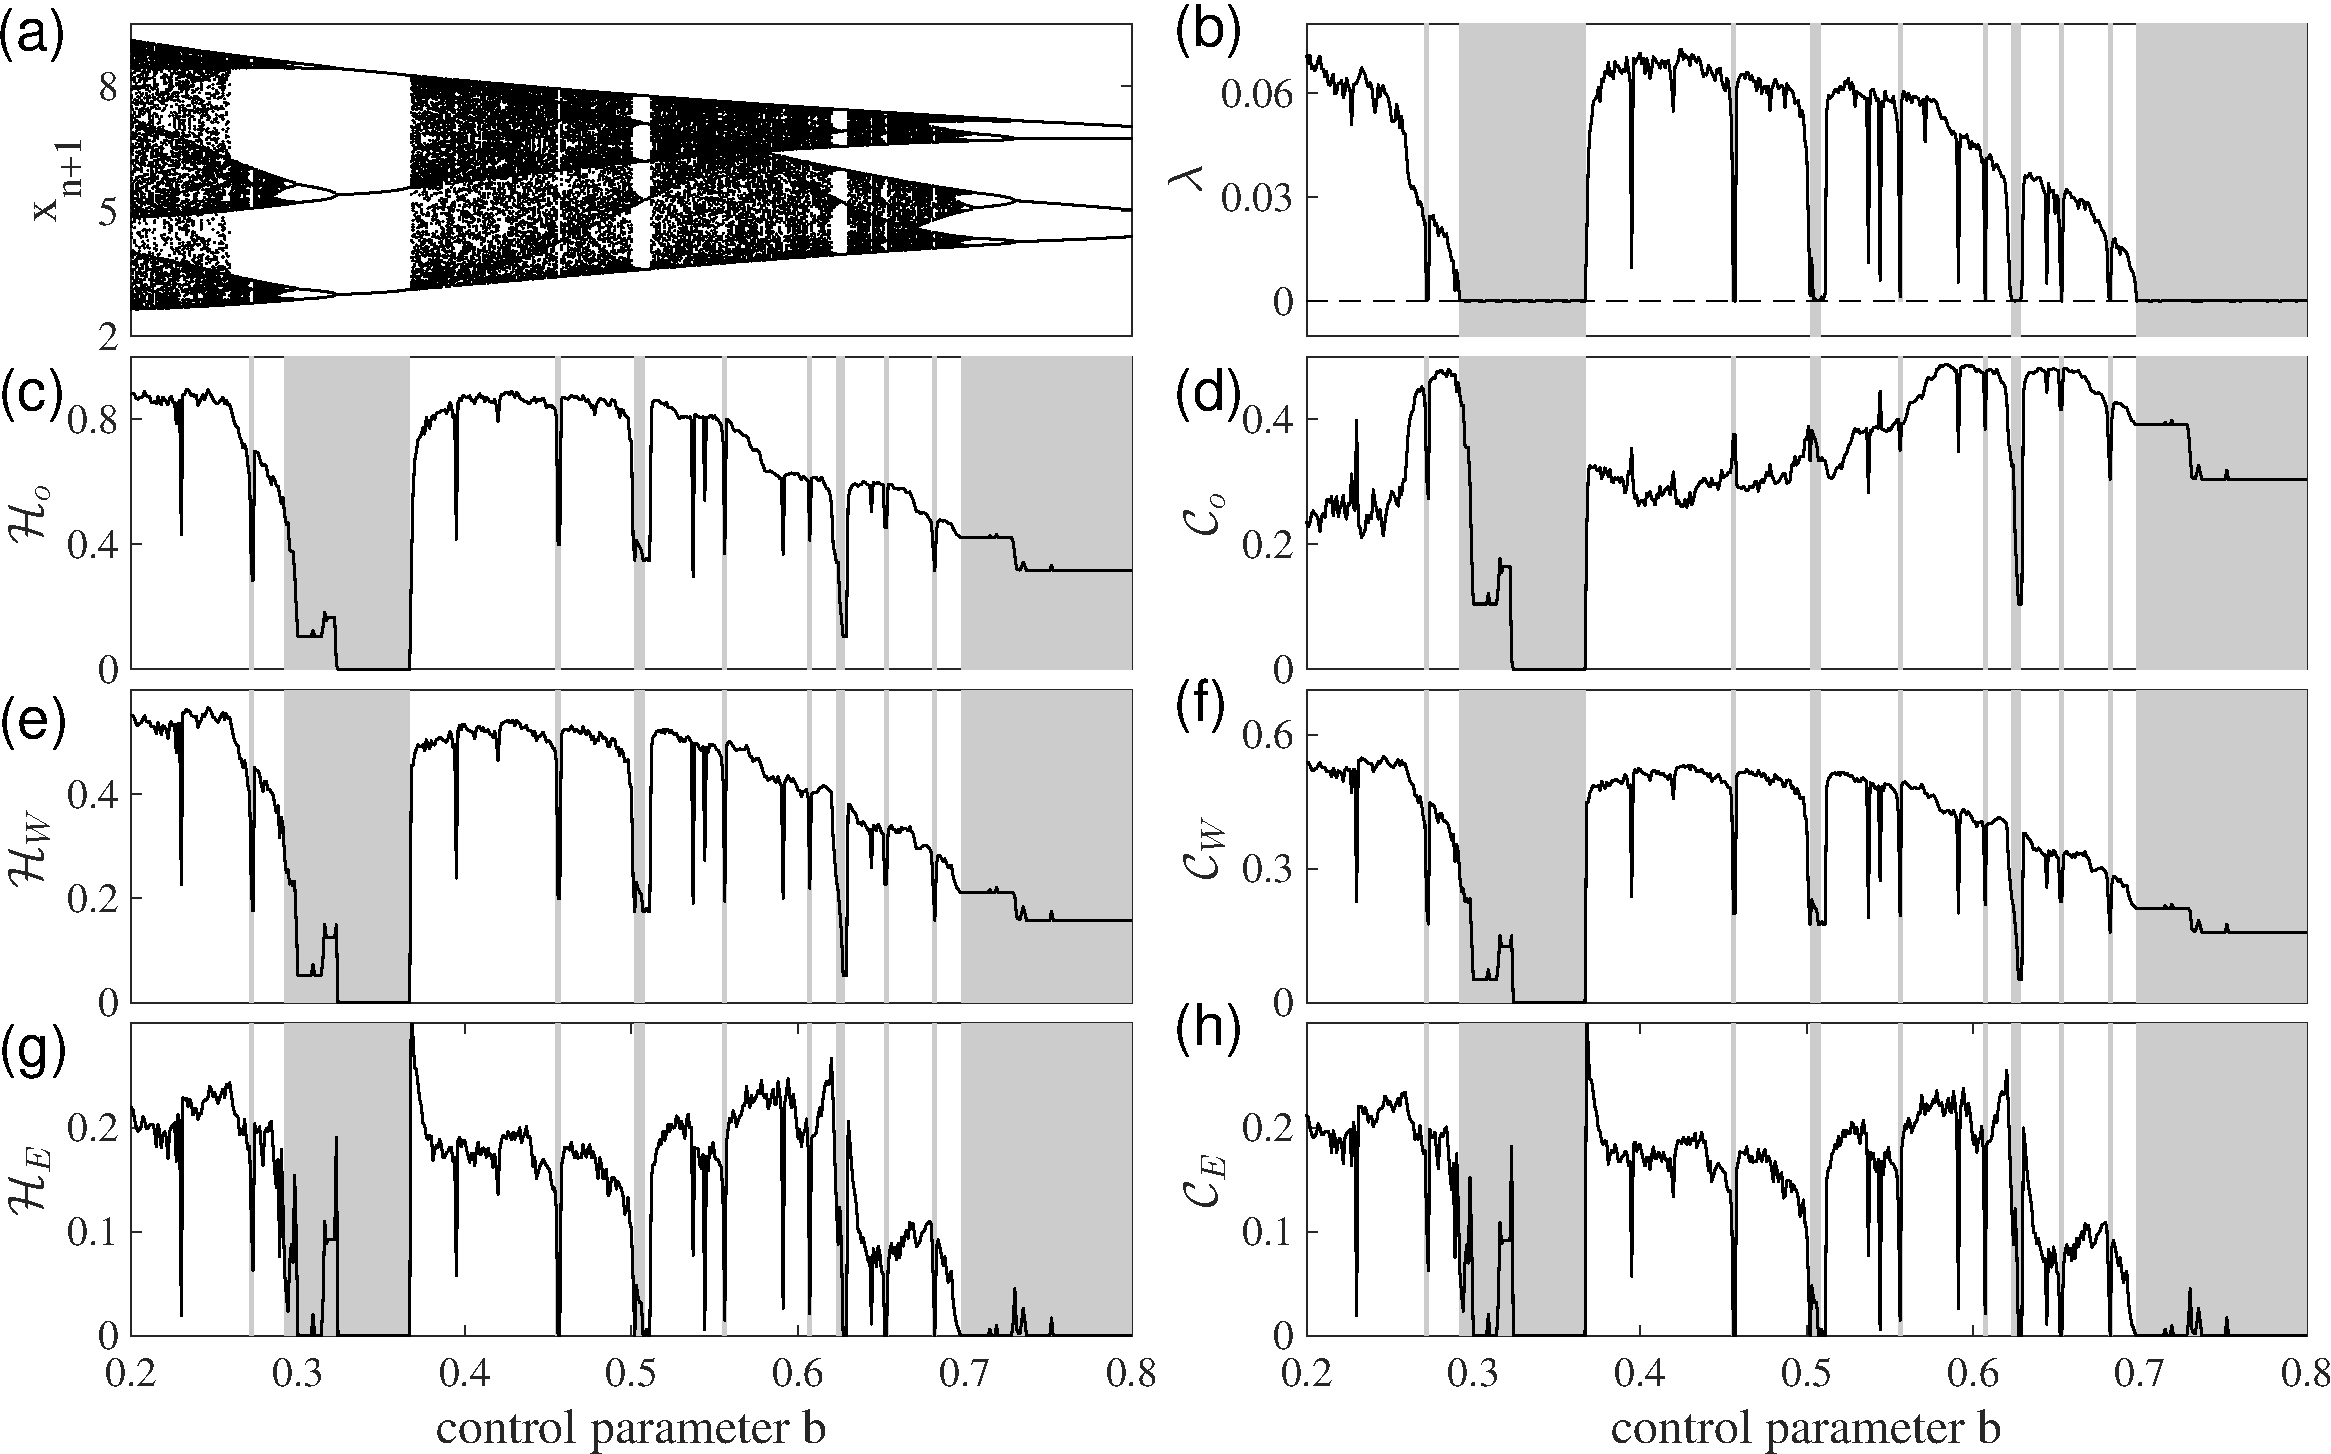
\includegraphics[width=2\columnwidth]{rosslerEntropy.pdf}
\caption{\small{Same as Fig. \ref{fig:bifurcation}, but for Poincar\'e sections of the R\"ossler system while varying the control parameter $b$ (see text for details). Panel (a) presents a bifurcation diagram based on the $x$ components of all points in the Poincar\'e sections. Panel (b) shows the largest Lyapunov exponent of the system in dependence of $b$.} \label{fig:bifurRossler}}
\end{figure*}


\section{Real-world examples} \label{sec:time}

While we have previously demonstrated the suitability of OPTN based SCMs for tracing changes in dynamical complexity for time series from deterministic dynamical systems, in the following we will use two different experimental time series to demonstrate that SCMs also successfully characterize the complexity properties of real-world systems, showing distinct values for different types of dynamics. 

The first example originates from a laboratory fluid experiment of baroclinic instability which is used to study patterns of cyclones and anticyclones in the Earth's atmosphere~\cite{Read_jfm_1992,ZouEPJST2008}. Depending on the parameters rotation rate, temperature difference, viscosity and fluid density, this experimental system exhibits a rich variety of flow regimes. In particular, we focus on the following regimes: 
\begin{enumerate}[(i)]
\item {Stable fluid:} The temperature signal of the stable flow exhibits periodic oscillations as the wave drift patterns arrive at the measured fixed point. 
\item {Quasi-periodic 2-frequency amplitude vacillation (AV-2):} This case is identified as a 2-frequency quasi-periodic amplitude flux. The wave drift is composed of slow and regular oscillations in the temperature signal, but a fast modulation in the amplitude is also visible. AV-2 is characterized by a periodic growth and drop in wave amplitude with little change in waveform. 
\item {Quasi-periodic 3-frequency amplitude vacillation (AV-3):} We also analyze a quasi-periodic 3-frequency amplitude vacillation time series which is obtained from a three-dimensional direct numerical simulation in an air-filled rotating baroclinic instability experiment~\cite{Read_jfm_1992}. 
\item {Modulated amplitude vacillation (MAV):} This case is identified as a low-dimensional stream, chaotically modulated and with waves of varying amplitudes. Amplitude modulation results in a complex temperature signal.
\end{enumerate}

The second set of example time series comprises physiological signals of human electrocardiogram (ECG) recordings collected from patients in a Coronary Care Unit and the Creighton University Cardiac Center. Heart rate variability suffering from ventricular arrhythmia presents a physiologically highly significant but still relatively poorly understood dynamical system, showing rich nonlinear properties. In this work, we focus on three different states: normal sinus rhythm (SR), ventricular tachycardia (VT) and ventricular fibrillation (VF) \cite{smallCSF2002}. From the data bank of recordings of ECG during various rhythms, we selected 14 time series showing sinus rhythm (SR) prior to onset of arrhythmia, 12 time series of VT and 17 of VF. The ECG recordings have been annotated with SR, VT and VF by skilled cardiologists on the basis of waveform morphology. Each recording consists of at least $10,000$ data points (20~s) in length at a 250~Hz sampling frequency. 

For choosing the embedding parameters for both sets of example time series, we follow the suggestions from earlier studies~\cite{ZouEPJST2008,smallCSF2002}. Although we are facing the inevitable presence of nonstationarity and noise in the experimental data, we have verified that the following results do not change significantly while our embedding parameters are varied. In particular, we have treated the embedding dimension as a free parameter which has been varied in the range of $D = 2, 3, \ldots, 7$, while the embedding delay $\tau$ has been kept fixed as follows. In the case of temperature time series from the fluid experiments, $\tau_{i} = 218$~s for the stable solution, $\tau_{ii} = 136.5$~s  for AV-2, $\tau_{iii} = 185.625$~s for AV-3, and $\tau_{iv} = 118$~s for MAV. For the ECG time series, we consistently use an embedding delay of $\tau = 5$. The results have been averaged over all subjects. 

In both sets of time series, the OPTN based SCMs enhance our understanding of the underlying nonlinear system, which can be seen from the results summarized in Fig.~\ref{fig:fluid}. In the case of the fluid data (Fig.~\ref{fig:fluid}(a)), $\mathcal{H}_O$, $\mathcal{H}_W$, $\mathcal{C}_W$, $\mathcal{H}_E$ and $\mathcal{C}_E$ all show consistent changes of the complexity and entropy values between stable wave solution (SW), quasi-periodic 2-frequency amplitude vacillation (AV-2), quasi-periodic 3-frequency amplitude vacillation (AV-3) and chaotic modulated amplitude vacillation (MAV). Specifically, the complexity of these four cases has the following order: SW has the smallest complexity since it shows periodic oscillations with trivial recurrence, while MAV has the highest complexity since it presents chaotically modulated amplitude vacillation. Quasiperiodic states show intermediate complexity values since these two cases have non-trivial recurrences but with low complexity. Interestingly, AV-3 presents higher complexity than AV-2. The order of complexity values between periodic, quasiperiodic and chaotic solutions still holds for $\mathcal{C}_O$ although the corresponding values become comparable. In particular, it becomes hard for $\mathcal{C}_O$ to identify the difference between AV-2 and AV-3. 

Qualitatively similar results are obtained for the ECG recordings (Fig.~\ref{fig:fluid}(b)). Clearly, different ECG recordings exhibit remarkably distinct complexity values. Specifically, SR recordings show very pronounced the highest values of $\mathcal{H}_O$, $\mathcal{H}_W$, $\mathcal{C}_W$, $\mathcal{H}_E$ and $\mathcal{C}_E$, reflecting the existence of significant spectral power in a rather broad frequency band between 50 and 100 beats/min in the signals \cite{smallCSF2002}. On the other hand, the complexity of VT has the smallest value, even lower than for the case of VF. Unlike the other five measures, we note, however, that SR shows the smallest value of $\mathcal{C}_O$ while VT and VF have comparable values that are higher than SR. This difference may be explained by the fact that unlike the two other OPTN based SCMs, this measure only takes static information of pattern frequencies into account and may therefore not be able to properly distinguish subtle differences reflected in the temporal order of patterns.

\begin{figure*}
	\centering 
	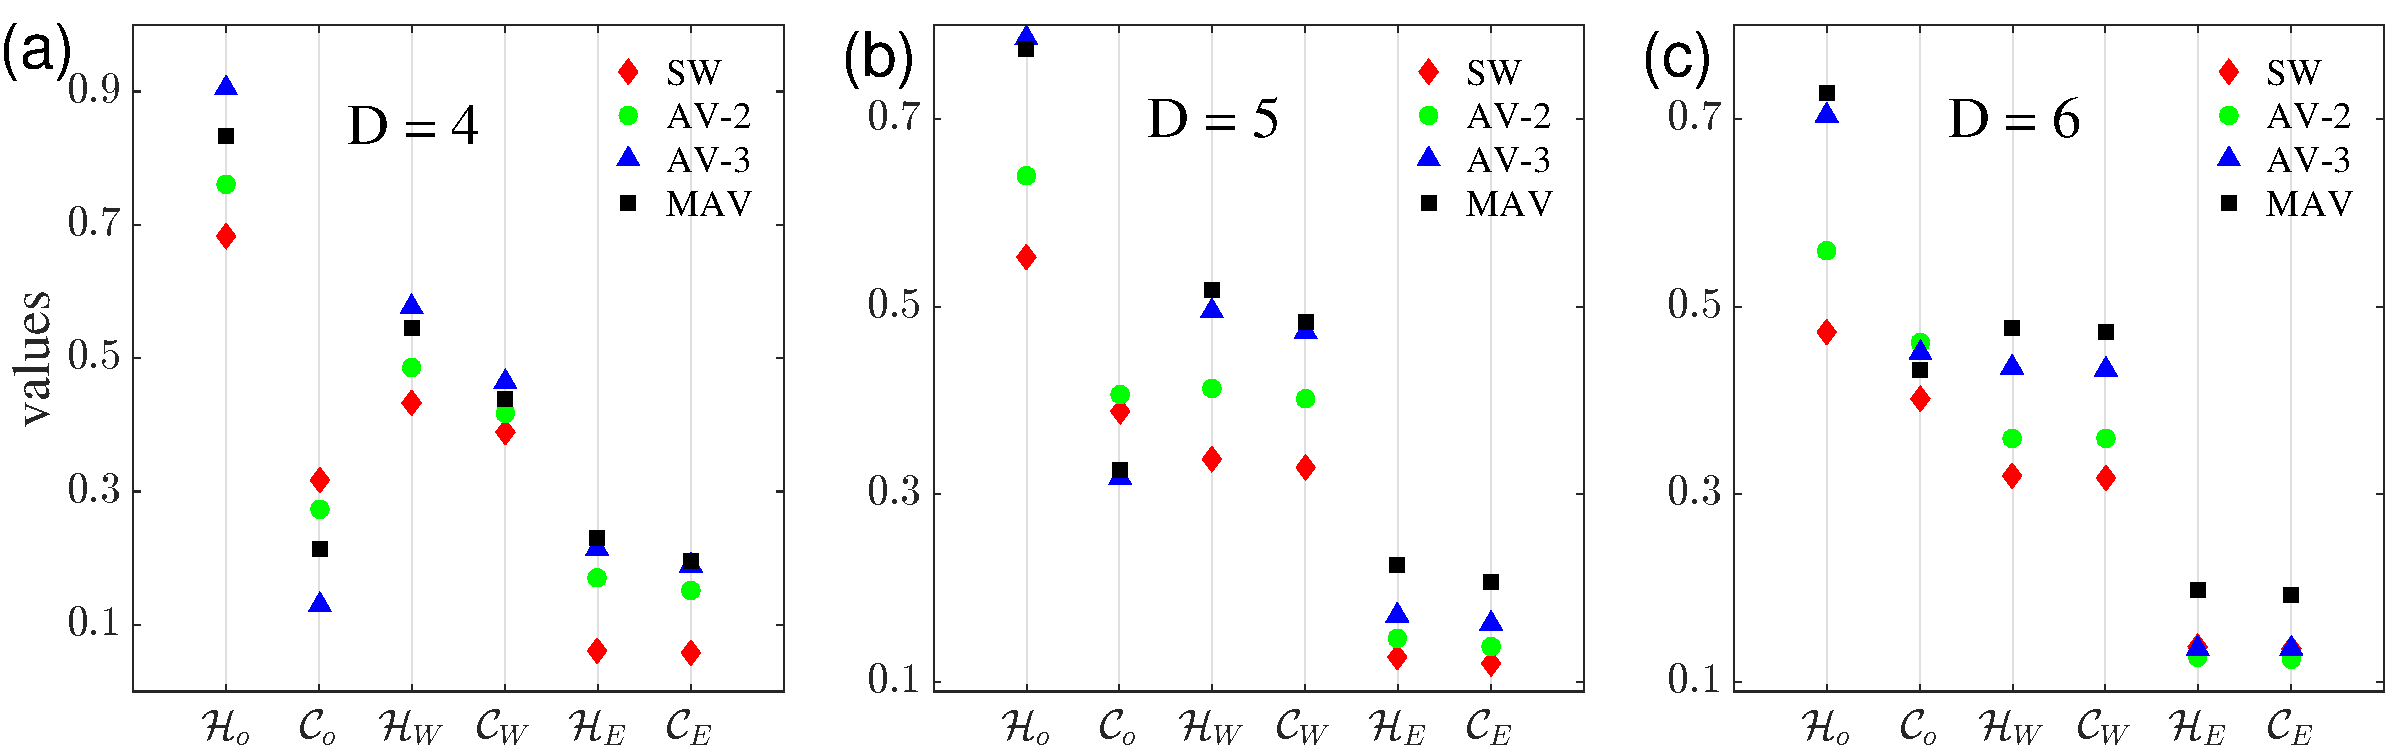
\includegraphics[width=2\columnwidth]{fluidExample.pdf}
\caption{\small{OPTN based entropy and SCM characteristics for experimental fluid data (a) and human ECG recordings (b). The results have been averaged over embedding dimensions in the range of $D = 2, 3, \ldots, 7$. In (a), stable wave (SW, $\blacklozenge$), quasiperiodic 2-frequency amplitude vacillation (AV-2, $\bullet$), quasiperiodic 3-frequency amplitude vacillation (AV-3, $\blacktriangle$) and chaotic modulated amplitude vacillation (MAV, $\blacksquare$) are distinguished. In (b), results are shown for normal sinus rhythm (SR, $\blacktriangle$), ventricular tachycardia (VT, $\blacklozenge$) and ventricular fibrillation (VF, $\bullet$). } \label{fig:fluid}}
\end{figure*}


\section{Conclusions} \label{sec:con}
In summary, we have proposed to expand the traditional ordinal pattern frequency analysis by also including ordinal pattern transitions, thereby generalizing existing statistical complexity measures for nonlinear time series analysis. The pattern transition properties encoded in the underlying time series networks provide novel insights beyond that provided by the celebrated permutation entropy which relies on the pattern frequencies only. Therefore, this study presents another case showing the usefulness of applying ordinal pattern transition networks for time series analysis \cite{ZouPR2018}. 

We have suggested two slightly different ways to consider the effects of pattern transitions in statistical complexity measures, which are based on (i) a globally normalized transition matrix and (ii) a node-wise normalized transition matrix. Here, the complexity measure based on the node-wise normalized matrix considers both, individual pattern frequencies and the frequencies of transitions among patterns. We have shown that the associated two new statistical complexity measures characterize the complexity properties of deterministic chaos successfully and clearly highlight deterministic-chaotic dynamics in the corresponding complexity--entropy planes (Fig.~\ref{fig:CElogistic}). This finding helps to obtain an improved complexity analysis for time series of both deterministic chaos and stochastic systems, fostering their better understanding. However, further more systematic numerical performance tests employing different types of dynamical systems are required to provide compelling evidence for distinctions between different dynamics beyond the cases presented in the current work, including various models of chaotic maps, long-range correlated stochastic processes like fractional Brownian motion and fractional Gaussian noise, etc.~\cite{BorgesAMC2019,RossoPRE2007}. While this opens several opportunities for follow-up research, we have demonstrated here the practical usefulness of our improved SCMs by employing this framework to time series for experimental fluid flows and ECG recordings, showing distinctive characteristics for different dynamics. 

Some open problems common to other nonlinear time series analysis methods remain to be further addressed in future work, for example, the dependence of reliable estimates of SCMs on the available time series lengths. For time-discrete dynamical systems like chaotic maps, one may easily use longer data series, which however does not improve the estimate very much due to the accumulation of effects due to a limited numerical precision (Fig.~\ref{fig:transient}). For continuous systems, together with the embedding parameters, the sampling frequency is another important characteristic which needs to be further explored. Moreover, the generalization of our approach from univariate to bivariate time series analysis shall be further discussed. We noticed that this aspect has remained a largely untouched subject for statistical complexity analysis so far, while it presents an interesting task to show the dependence of complexity on interaction. 
%Finally, this work has focused on complexity measures exploiting the classical notion of Shannon entropy in various ways. In turn, a plethora of dynamical systems exhibiting particularly complex behavior may present multifractal characteristics and would therefore benefit from considering the full spectrum of generalized (R\'enyi) entropies and associated statistical complexity measures to completely capture the information on dynamical complexity encoded in ordinal pattern sequences. 
We outline further work on the aforementioned topics as subjects of future research.

\section*{Acknowledgements}
Parts of this work have been financially supported by the National Natural Science Foundation of China (grant no. 11872182 and 11835003). YZ further acknowledges support by the Shanghai Municipal Science and Technology Major Project (grant no. 2018SHZDZX01) and ZJ Lab. 

\bibliographystyle{unsrt}
\bibliography{ref_Zou,ref_Donner}

\end{document}
